
%\documentclass[a4paper, titlepage]{report}
\documentclass[ALICE,manyauthors]{cernphprep}

%\usepackage{textcomp}
\usepackage[english]{babel}
\usepackage{fancyhdr}
\usepackage{amsmath}
\usepackage{graphicx}
\usepackage{verbatim}
\usepackage{lineno}
\usepackage{amsfonts}
\usepackage{makeidx}
\usepackage{color}
\pagestyle{headings}
\usepackage{epstopdf}
\usepackage{multirow}
\usepackage{hyperref}   % creates links to references, chapters etc and a separated table of contents in the .pdf file

%%%
%%% Alias
%%%
\newcommand{\pp}{p-p}
\newcommand{\sqrts}{\sqrt{s}}
\newcommand{\sqrtsNN}{\sqrt{s_{\rm \scriptscriptstyle NN}}}
\newcommand{\lsim}{\,{\buildrel < \over {_\sim}}\,}
\newcommand{\gsim}{\,{\buildrel > \over {_\sim}}\,}
\newcommand{\av}[1]{\left\langle #1 \right\rangle}
\newcommand{\eV}{\mathrm{eV}}
\newcommand{\keV}{\mathrm{keV}}
\newcommand{\MeV}{\mathrm{MeV}}
\newcommand{\GeV}{\mathrm{GeV}}
\newcommand{\TeV}{\mathrm{TeV}}
\newcommand{\ev}{\mathrm{eV}}
\newcommand{\kev}{\mathrm{keV}}
\newcommand{\mev}{\mathrm{MeV}}
\newcommand{\gev}{\mathrm{GeV}}
\newcommand{\tev}{\mathrm{TeV}}
\newcommand{\fm}{\mathrm{fm}}
\newcommand{\mm}{\mathrm{mm}}
\newcommand{\cm}{\mathrm{cm}}
\newcommand{\m}{\mathrm{m}}
\newcommand{\mum}{\mathrm{\mu m}}
\newcommand{\s}{\mathrm{s}}
\renewcommand{\d}{\mathrm{d}}
\newcommand{\ns}{\mathrm{ns}}
\newcommand{\mrad}{\mathrm{mrad}}
\newcommand{\mb}{\mathrm{mb}}
\newcommand{\mub}{\mathrm{\mu b}}
\newcommand{\T}{\mathrm{T}}
\newcommand{\PbPb}{\mbox{Pb--Pb}}
\newcommand{\Npart}{N_{\rm part}}
\newcommand{\Ncoll}{N_{\rm coll}}
\newcommand{\Raa}{R_{\rm AA}}
\newcommand{\RAA}{R_{\rm AA}}
\newcommand{\TAA}{T_{\rm AA}}
\newcommand{\RCP}{R_{\rm CP}}
\newcommand{\pt}{p_{\rm T}}
\newcommand{\dNdy}{{\rm d}N_{ch}/{\rm d}y}
\newcommand{\momwin}{[$p$, $p$+$\Delta$ $p$]}
\newcommand{\DtoKpi}{{\rm D^0\to K^-\pi^+}}
\newcommand{\DtoKpipi}{{\rm D^+\to K^-\pi^+\pi^+}}
\newcommand{\DstartoDpi}{{\rm D^{*+}\to D^0\pi^+}}
\newcommand{\Dzero}{{\rm D^0}}
\newcommand{\Dstar}{{\rm D^{*+}}}
\newcommand{\Dplus}{{\rm D^+}}
\newcommand{\nbinv}{{\rm nb^{-1}}}
\newcommand{\decleng}{{\rm L}_{xyz}}
\newcommand{\dEdx}{{\rm d}E/{\rm d}x}
\newcommand{\mufac}{\mu_{\rm F}}
\newcommand{\muren}{\mu_{\rm R}}
\newcommand{\fprompt}{f_{\rm prompt}}
%%%
%%% end Alias
%%%

\begin{document}
\begin{titlepage}


%\PHnumber{ALICE-2011-XYZ}                 % required, obtained from PH
\PHdate{\today}              % required

\title{D-hadron correlations  in p-Pb collisions at $\sqrt{s_\mathrm{NN}}$ = 5.02 TeV}

\Collaboration{F. Colamaria, S. Kumar, M. Mazzilli}%

\ShortAuthor{DRAFT \today, FOR INTERNAL USE ONLY}
\ShortTitle{D-hadron correlations}

\begin{abstract}
In this note, we present the analysis of azimuthal correlations of D mesons and primary charged $\pi$,K,p,e,$\mu$ performed in the ALICE central barrel in p-Pb collisions at $\rm{\sqrt{s_{NN}}}$ = 5.02 TeV, from 2016 data taking. The analysis is performed in an extended $\pt$ range and with additional observables with respect to p-Pb 2013 data analysis. After a description of the analysis strategy, corrections and systematic uncertainties, the results obtained for prompt $\Dzero$, $\Dstar$ and $\Dplus$mesons in different ranges of transverse momentum of the D meson and of the associated particles are presented. The results are then compared to Monte Carlo models and also with published 2013 p-Pb analysis results for the common $\pt$ ranges. 
The first section of the note deals with the centrality-integrated analysis; the second is focused on the analysis as a function of the ZNA centrality.
\end{abstract}


\end{titlepage}

\linenumbers
\tableofcontents

\newpage
\section{Introduction and Motivation}
%Two-particle azimuthal correlations in different kinematic ranges have played a crucial role in the understanding of jet production
%and modification in relativistic heavy-ion collisions, from RHIC to LHC energies.
%The extension of these studies to the heavy-flavour domain at the LHC will probe our understanding of QCD in the perturbative
%regime, accessible in a large kinematic range given the large mass of heavy quarks. Flavour conservation in QCD implies that charm quarks5are always produced as pairs of quarks and anti-quarks. The azimuthal correlations obtained using a meson carrying a heavy quark as trigger particle
%with the other charged particles in the same event give the possibility to study the underlying charm production mechanism in detail. In particular, prompt
%heavy quark pair production leads, at first order in leading-order pQCD, to back-to-back production. Heavy quarks produced by splitting of massless gluons are instead
% produced at small $\Delta\phi$. A third production process, the production
%by flavour excitation leads to a big separation in rapidity and most of the time one of the two quarks is produced in the forward region. \\

%Angular differential measurements of charm production are therefore interesting in their own right in pp collisions to study the structure
%and fragmentation of charm quarks, as well as their production mechanism. Correlations of  prompt charm meson pairs were first measured by Fermilab E791 Collaboration at Tevatron \cite{E791} also later by
%CDF II at Tevatron, showing a fair agreement with Pythia for the overall production, with some disagreement in the collinear and back-to-back production~\cite{CDF}. \\

%Heavy-flavour correlation studies in more complex collisional systems, like Pb-Pb aim to study the modification of the fragmentation of charmed jets due to in-medium (or cold nuclear matter, in case of p-Pb collisions) effects, in a similar fashion as it was done for di-hadron correlation studies in heavy-ion collisions (see for example~\cite{th1,th2}). Furthermore, the recent observation of long range correlations in p-Pb for light flavour hadrons and for heavy-flavour decay electrons %add reference
%points to possible collective effects or effects originating from gluon saturation in the initial state. More information could be extracted by the eventual observation of the same effect with D mesons.\\

%In the following, we describe the analysis strategy for p-Pb in all its steps, and we describe the list of corrections and the estimation of the systematic uncertainties
%done. After a section dedicated to detailed studies performed with Monte Carlo simulations to check the different analysis steps, we present the results of
%$\Delta\phi$ correlations obtained for prompt $D^0$, $D^{+}$ and $D^{*+}$ in different ranges of transverse momentum for the D-meson (trigger particle) and the associated particles.

The study of the azimuthal correlations of heavy-flavour particles and charged particles at the LHC energies provides a way to characterize charm production and fragmentation processes in pp collisions. The measurement also provide a way to probe our understanding of QCD in the perturbative regime, accessible in a large kinematic range given the large mass of heavy quarks. Flavour conservation in QCD implies that charm quarks are always produced as pairs of quarks and anti-quarks. The azimuthal correlations obtained using a meson carrying a heavy quark as trigger particle with the other charged particles in the same event give the possibility to study the underlying charm production mechanism in detail. In particular, prompt charm quark-antiquark pair production is back to back in azimuth at first order in leading-order perturbative-QCD (pQCD). If a hadron from the quark hadronization is taken as trigger particle, a near-side (at $\Delta\varphi = 0$) and an away-side (at $\Delta\varphi = \pi$) peaks would appear in the azimuthal correlation distributions, coming from the fragmentation of the quark pair. Heavy quarks produced from the splitting of a massless gluon can be rather collimated and may generate sprays of hadrons at small $\Delta\varphi$. Finally, for hard-scattering topologies classified as ``flavour-excitation", a charm quark undergoes a hard interaction from an initial splitting ($g\to c\bar{c}$), leading to a big separation in rapidity of the hadrons originating from the antiquark (quark) with respect to the trigger D meson and contribute to a rather flat term to the $\Delta\varphi$-correlation distribution.

Heavy-flavour correlation studies in more complex collision systems, like Pb-Pb, play a crucial role in studying the modification of the fragmentation of charmed jets due to in-medium (or cold nuclear matter, in case of p-Pb collisions) effects, in a similar way as it was done for di-hadron correlation studies in heavy-ion collisions (see for example \cite{ALICEPbPbdih}). Furthermore, the recent observation of long range correlations in p-Pb for light flavour hadrons (\cite{ALICEv2ppb}, \cite{ALICEv2ppb2}) and for heavy-flavour decay electrons (\cite{ALICEv2HFe}) points to possible collective effects or effects originating from gluon saturation in the initial state. More information could be extracted by the eventual observation of the same effect with D mesons.\\

In the following note, we first describe the analysis strategy for the p-Pb 2016 data sample in all its steps, followed by the list of analysis corrections and the estimation of systematic uncertainties. Finally the results of $\Delta\varphi$ correlations, and quantitative observable extracted to fits to those distributions, obtained for prompt $\rm{D^0}$, $\rm{D^{+}}$ and $\rm{D^{*+}}$ in different ranges of transverse momentum for the D-meson (trigger particle) and the associated particles are presented.

The extension of the momentum ranges (both for D mesons and associated particles) with respect to the 2013 p-Pb dataset, as well as the improved precision in the common ranges allow a more thorough investigation of the charm quark fragmentation properties (multiplicity of tracks as a function of momentum, geometrical profile of charm jets, $\pt$ distribution of the tracks inside the jet). This can also allow us to put better constraints on the description of charm fragmentation and charm jet properties provided by models.
The possibility of spotting cold nuclear matter effects affecting the charm fragmentation in p-Pb was severely limited, in the published paper, by the uncertainties on both pp and p-Pb samples. This will no longer be the case with the new p-Pb data sample, as soon as a pp sample with equivalent precision is collected (the pp reference run expected by the end of this year could be of help in this sense).
In addition, the new measurements can be used as solid and precise references in view of an analysis on a Pb-Pb sample at the same energy (hopefully already in 2018 data taking, otherwise after the ALICE upgrade).


\newpage
\section{Data/Monte Carlo samples and event selection}
The data used for the analyses were the AOD samples of the following four datasets: LHC16q$\_$FAST, LHC16q$\_$CENT$\_$woSDD, LHC16t$\_$FAST, LHC16t$\_$CENT$\_$woSDD. The reason for choosing these data samples (in particular, those without the drifts for the CENT cluster) is explained later on, in this section. It was verified, by looking at D-meson and associated charged track $\eta$ and $\varphi$ distributions, and at the mixed-event correlation distributions for each subsamples, that no visible differences is present for the four periods, hence it was possible to perform the analysis directly on the merged samples without any bias.

The Monte Carlo productions adopted for this study were:
 \begin{enumerate}
 \item LHC17d2a$\_$fast$\_$new, a HIJING production with enrichment of heavy quarks (charm and beauty) and their decay products in each of the event, performed by PYTHIA6 with Perugia2011 tune, and with forced hadronic decays of the charmed hadrons. This production was used for D-meson efficiency evaluation, purity estimation and Monte Carlo closure test.
 \item LHC17f2b$\_$cent$\_$woSDD and LHC17f2b$\_$fast, minimum-bias samples produced with DPMJET generator, are used for the evaluation of the tracking efficiencies.
\end{enumerate}

Table 1 shows the list of runs used for the analysis, for each of the data taking periods, and of the Monte Carlo productions used to evaluate the corrections:

% Systematic table
\begin{table}[h]
\begin{tabular}{ p{1.2cm} | p{4.2cm} |  p{7cm} |  p{1.2cm}}
{\normalsize \textbf {Type}} &       {\normalsize \textbf {Production}} &       {\normalsize \textbf {Run list}} & {\normalsize \textbf {nEvents}} \\
\\ \hline
Monte-Carlo & LHC17d2a$\_$fast$\_$new (c/b enriched), LHC17f2b$\_$fast (MB), LHC17f2b$\_$cent$\_$woSDD (MB) &267166, 267165, 267164, 267163, 265525, 265521, 265501, 265500, 265499, 265435, 265427, 265426, 265425, 265424, 265422, 265421, 265420, 265419, 265388, 265387, 265385, 265384, 265383, 265381, 265378, 265377, 265344, 265343, 265342, 265339, 265338, 265336, 265335, 265334, 265332, 265309 = \textbf{[36 runs]} & 50M\\
\\ \hline

\multirow{7}{*}{} Data&LHC16q, pass1$\_$CENT$\_$woSDD & 265525, 265521, 265501, 265500, 265499, 265435, 265427, 265426, 265425, 265424, 265422, 265421, 265420, 265419, 265388, 265387, 265385, 265384, 265383, 265381, 265378, 265377, 265344, 265343, 265342, 265339, 265338, 265336, 265335, 265334, 265332, 265309 = \textbf{[32 runs]}& 261M total\\
                  &LHC16q, pass1$\_$FAST &265525, 265521, 265501, 265500, 265499, 265435, 265427, 265426, 265425, 265424, 265422, 265421, 265420, 265419, 265388, 265387, 265385, 265384, 265383, 265381, 265378, 265377, 265344, 265343, 265342, 265339, 265338, 265336, 265335, 265334, 265332, 265309 = \textbf{[32 runs]} & 260M \\
% \\ \hline
 & LHC16t, pass1$\_$CENT$\_$woSDD & 267166, 267165, 267164, 267163 = \textbf{[4 runs]} & 40M \\
% \\ \hline
  & LHC16t, pass1$\_$FAST & 267166, 267165, 267164, 267163 = \textbf{[4 runs]} & 41M \\
 \hline \hline
\label{tab:Sample}
\end{tabular}
\\
\caption {Data Set and Run list}
\end{table}

The trigger mask request for the event selection is kINT7. Only events with a reconstructed primary vertex within 10 cm from the centre of the detector along the beam line are considered. This choice maximises the detector coverage of the selected events, considering the longitudinal size of the interaction region, and
the detector pseudorapidity acceptances. In the analysis, the center-of-mass reference frame of the nucleon-nucleon collision is shifted in rapidity by $y_{\rm NN}$ = 0.465 in the proton direction with respect to the laboratory frame, due to the different per-nucleon energies of the proton and the lead beams.
Beam-gas events are removed by offline selections based on the timing information provided by the V0 and the Zero Degree Calorimeters, and the correlation between the number of hits and track segments in the SPD detector. This is automatically performed in the Physic Selection, a positive outcome of which is required during our event selection. The pile-up cuts for out-of-bunch pile-up protection are also invoked when calling the Physics Selection task.
The minimum-bias trigger efficiency is 100\% for events with D mesons with $\pt > 1$ $\gev/c$. For the analyzed data samples, the probability of pile-up from collisions in the same bunch crossing is below 2\% per triggered event (in most of the runs, well below 1\%). Events in which more than one primary interaction vertex is reconstructed with the SPD detector (with minimum of 5 contributors, and a $z$ distance greater than 0.8 cm) are rejected, which effectively removes the impact of in-bunch pile-up events on the analysis. Out-of-bunch tracks are effectively rejected by the Physics Selection pile-up cuts, and also by the request of at least one point in the SPD, which has a very limited time acquisition window (300 ns). Indeed, though the default associated track selection requires a minimum of 2 points in the ITS, as it will be shown later on full compatibility of the corrected results with 2 and 3 minimum ITS clusters are obtained. For FAST and CENT$\_$woSDD samples, the latter case indirectly forces the presence of a point in the SPD.

Since data collected during p-Pb 2016 data taking are distinguished into two categories - one including SDD detector (CENT$\_$wSDD sample) and the second one without the SDD in the reconstruction, or in the acquisition (CENT$\_$woSDD and FAST samples, respectively), a study of performance of the D-hadron correlation analysis with respect to the data samples employed has been carried out for $\Dstar$ and $\Dplus$ mesons (more sensitive to the presence of the SDD w.r.t. the $\Dzero$, due to their reconstruction from three decay tracks).

For this reason, the D-hadron correlation distribution has been compared on LHC16q$\_$pass1$\_$CENT$\_$wSDD and LHC16q$\_$pass1$\_$CENT$\_$woSDD and the relative statistical uncertainty has been estimated in the two cases. The goal was to understand if it was better to use the choose FAST and CENT$\_$woSDD samples, as it was ultimately done (which have the same detector conditions, and can be simply merged and considered, in the analysis chain, as a unique sample), of instead to use FAST and CENT$\_$wSDD samples (with different detector conditions, and hence requiring to perform the analysis separately on the two data sample, applying different corrections).
In particular, this study was crucial for the correlation analysis involving the $\Dstar$ meson, because the track reconstruction efficiency of the soft pion is $\approx 10\%$ higher employing also the SDD information.
Figure \ref{wSSvswoSDD} shows the normalized azimuthal correlation distribution for low, mid and high $\pt$ for $\Dstar$ meson. Blue points are referred to the woSDD sample while red points represents wSDD data. Figure \ref{wSSvswoSDDuncertainty} shows the relative statistical uncentainty extracted from the azimuthal correlation distributions for the $\Dstar$ in different kinematic ranges.

\begin{figure}[!h]
\centering
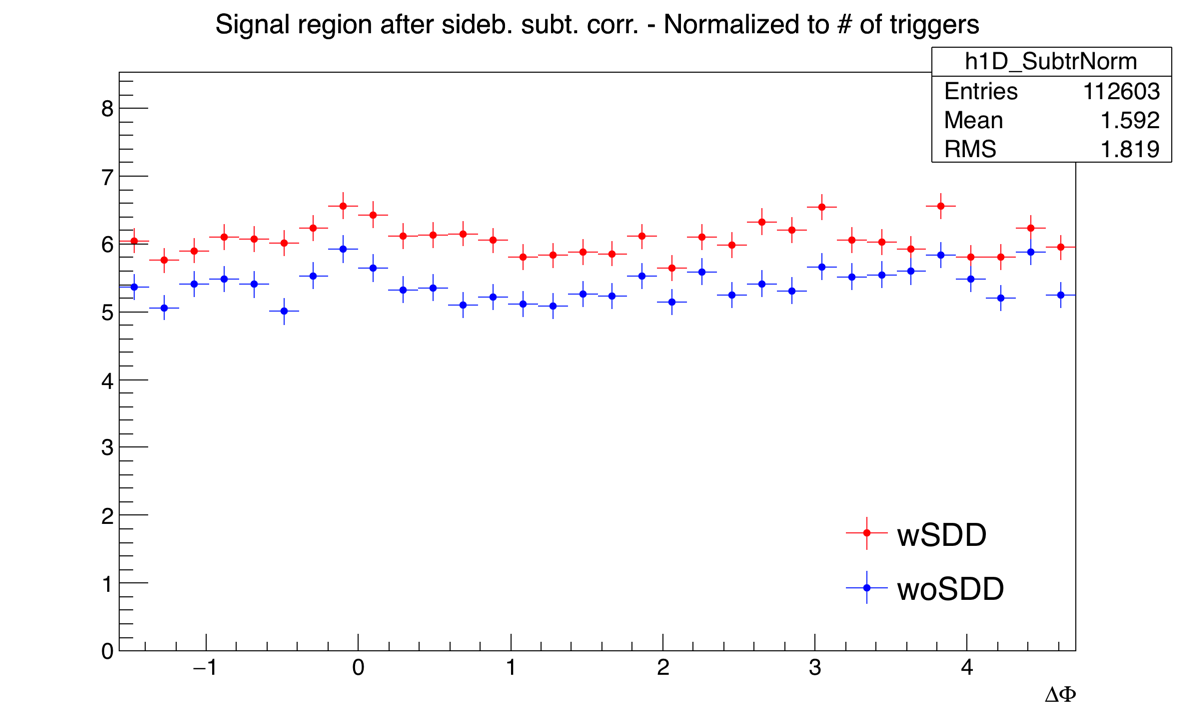
\includegraphics[width=0.8\linewidth, height=6cm]{figures/wSDD_vs_woSDD/AzimCorrDistr_Dstar_Canvas_PtIntBins2to3_PoolInt_thr0dot3to99dot0_Superimp.png}
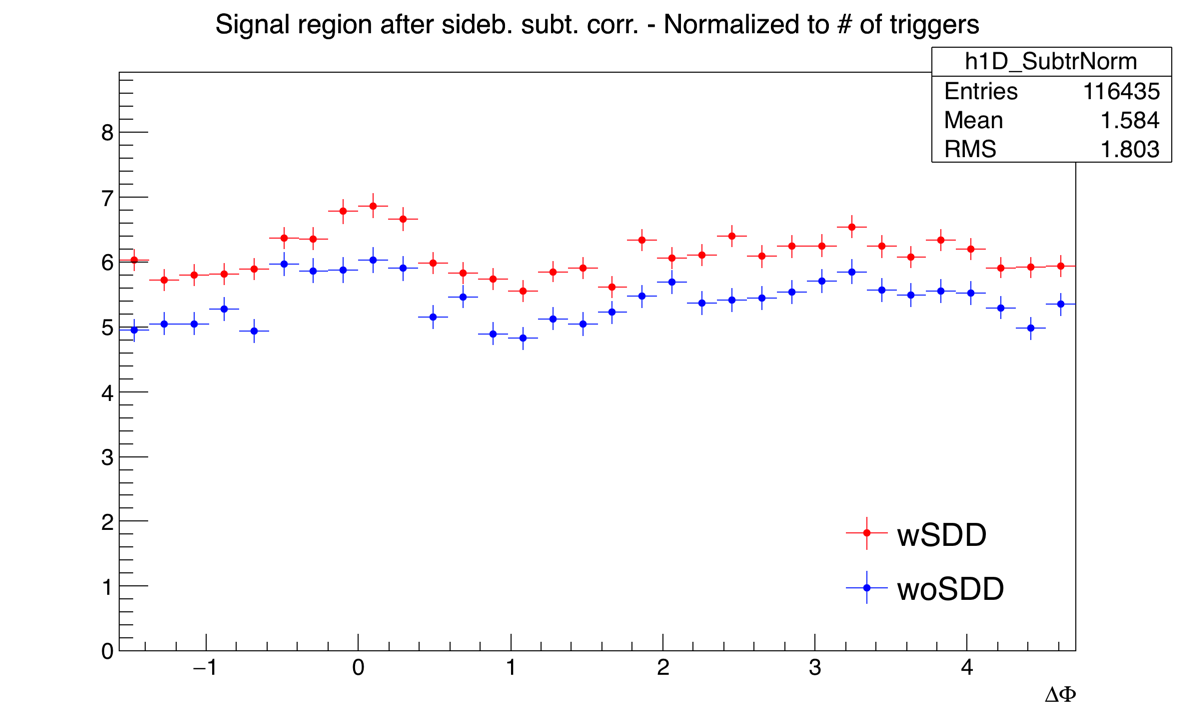
\includegraphics[width=0.8\linewidth, height=6cm]{figures/wSDD_vs_woSDD/AzimCorrDistr_Dstar_Canvas_PtIntBins4to6_PoolInt_thr0dot3to99dot0_Superimp.png}

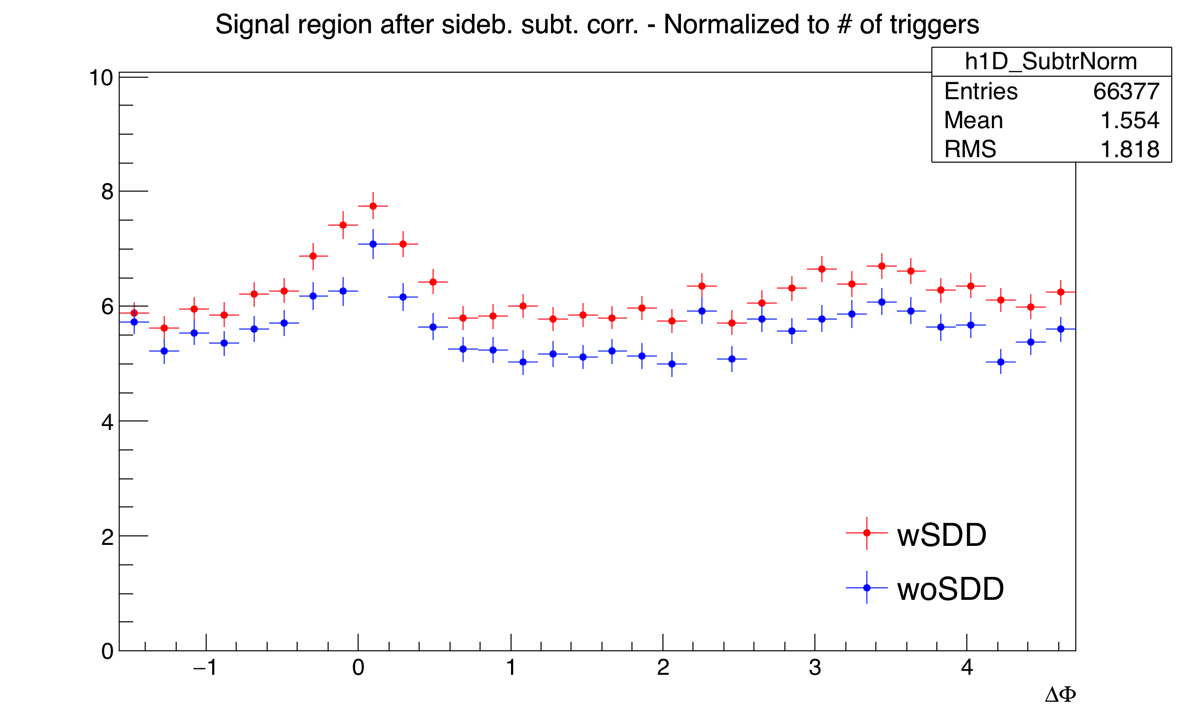
\includegraphics[width=0.8\linewidth, height=6cm]{figures/wSDD_vs_woSDD/AzimCorrDistr_Dstar_Canvas_PtIntBins7to9_PoolInt_thr0dot3to99dot0_Superimp.png}
\caption{Normalized azimuthal correlation distribution of $\Dstar$ for low $\pt$ ($3 < \pt(\Dstar) < 5$ $\gev/c$) on the top panel, mid $\pt$ ($5 < \pt(\Dstar) < 8$ $\gev/c$) on the middle panel and high $\pt$ ($8 < \pt(\Dstar) < 16$ $\gev/c$) on the bottom panel with a $\pt$ threshold for associated tracks of $\pt(assoc) > 0.3$ $\gev/c$. Blue points are referred to the woSDD sample while red points represent wSDD data.}
\label{wSSvswoSDD}
\end{figure}

\begin{figure}[!h]
\centering
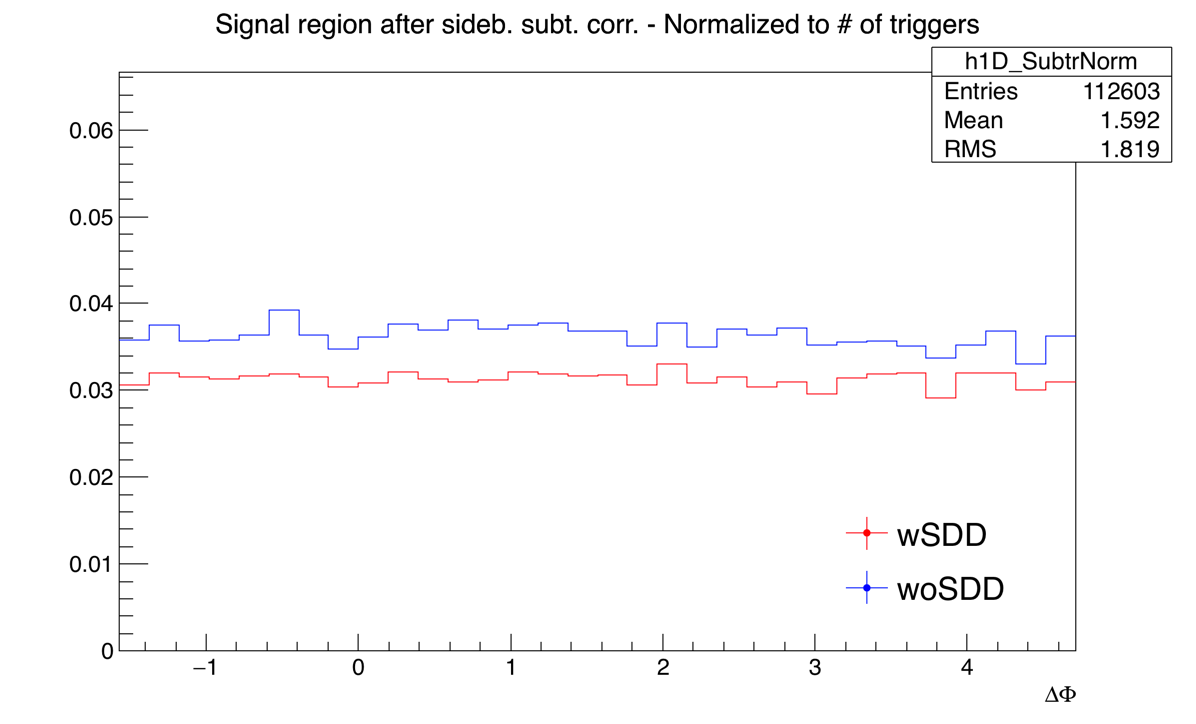
\includegraphics[width=0.8\linewidth, height=6cm]{figures/wSDD_vs_woSDD/Uncertanty_AzimCorrDistr_Dstar_Canvas_PtIntBins2to3_PoolInt_thr0dot3to99dot0.png}
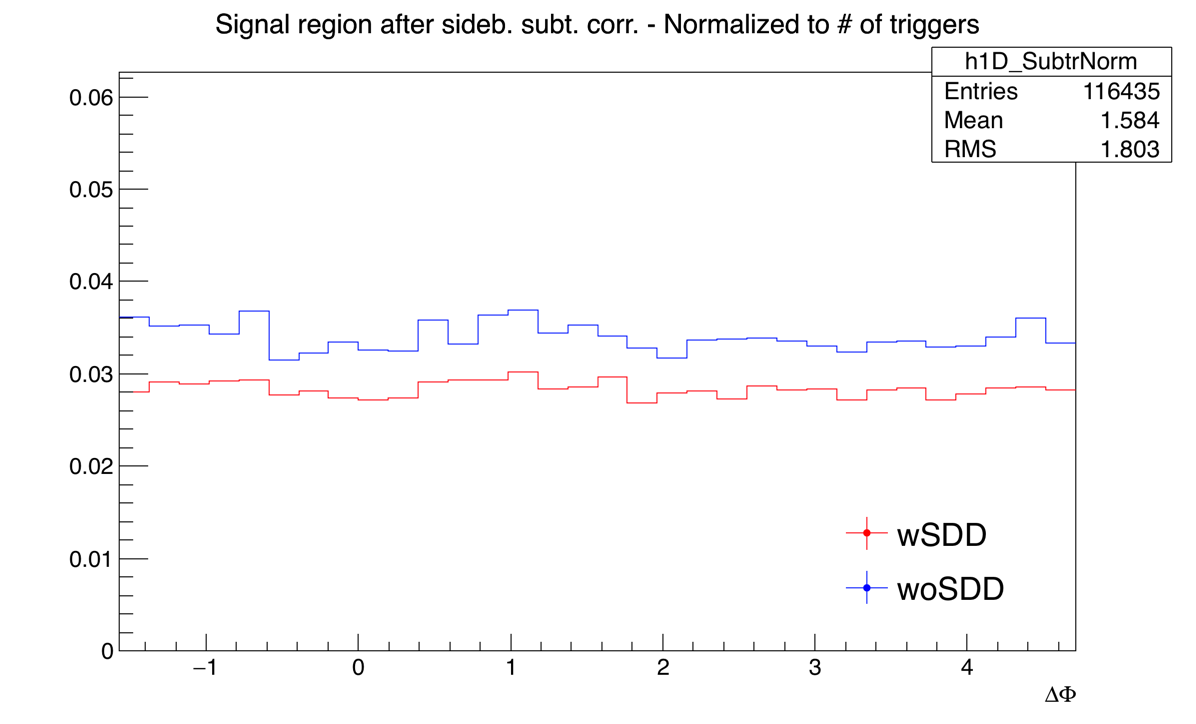
\includegraphics[width=0.8\linewidth, height=6cm]{figures/wSDD_vs_woSDD/Uncertanty_AzimCorrDistr_Dstar_Canvas_PtIntBins4to6_PoolInt_thr0dot3to99dot0.png}

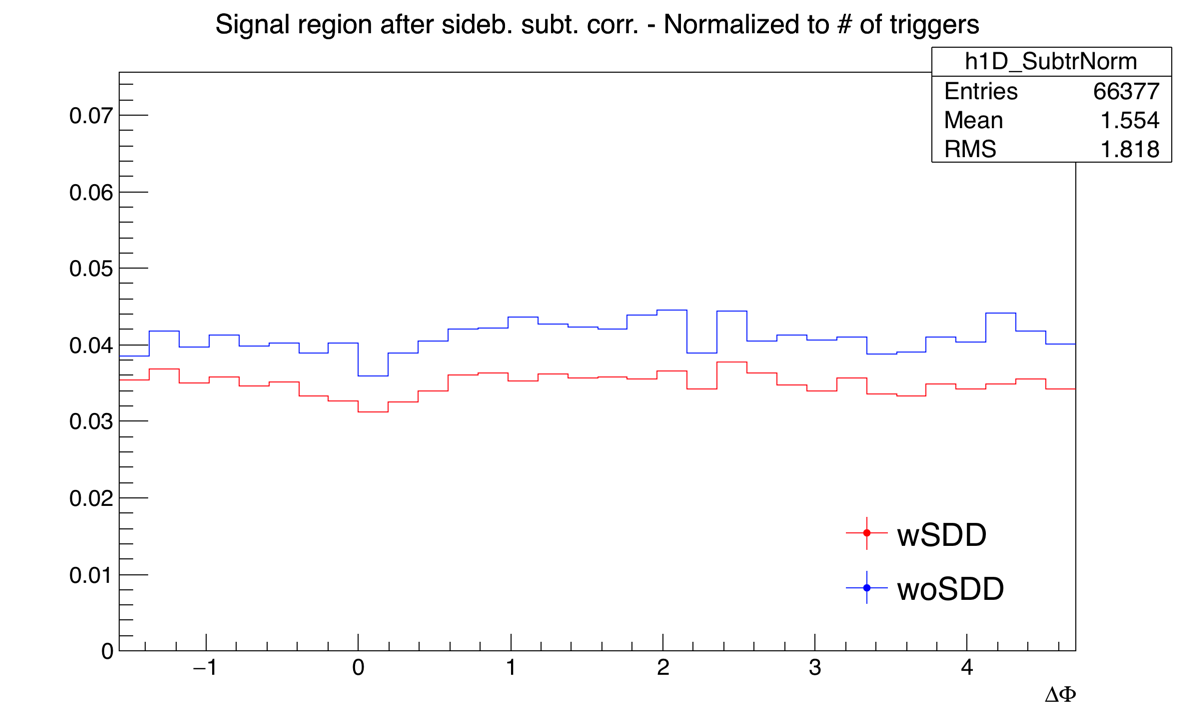
\includegraphics[width=0.8\linewidth, height=6cm]{figures/wSDD_vs_woSDD/Uncertanty_AzimCorrDistr_Dstar_Canvas_PtIntBins7to9_PoolInt_thr0dot3to99dot0.png}
\caption{Statistical uncertainty extracted from the azimuthal correlation distribution of $\Dstar$ with associated charged particles. Top panel: $3 < \pt(\Dstar) < 5$ $\gev/c$.
Mid panel: $5 < \pt(\Dstar) < 8$ $\gev/c$. Bottom panel: $8 < \pt(\Dstar) < 16$ $\gev/c$.
Blue line is referred to the woSDD sample while the red line represents wSDD data.}
\label{wSSvswoSDDuncertainty}
\end{figure}

It can be observed that the data sample that includes the SDD information is characterized by $\approx 10-15\%$ more statistics in each $\pt$ ranges analyzed. This difference is related to the larger efficiency in track reconstruction with the wSDD sample - a larger number of tracks survives to the selection request of 3 points in the ITS, which is part of the selection requests applied on the previous D-h analysis.

As a result, the wSDD sample is also affected by a slightly lower relative statistical uncertainty (about 12-15\%) due to several reasons: the larger tracking efficiency, the larger number of signal entries in the invariant mass distributions (again an effect of the larger tracking efficiency) and a slight increase of S/B, which reflects in a slight decrease of uncertainty from the sideband subtraction.
It has also to be considered that, on the full sample including also the FAST cluster, the increase in performance would be further reduced.
The overall statistical uncertainty difference resulting from the comparison is not enough to justify the implementation of two different analysis and two subsequent different corrections either for $\Dstar$ and $\Dplus$.

In order to, to cope with the lower tracking efficiency w.r.t. 2013 data sample, after this study, it was decided to reduce the ITS request for the associated tracks from 3 (used on 2013 data) to 2 ITS clusters as default selection criterion.




\newpage
\section{Analysis strategy}
The analysis follows the same strategy one used in 2013 p-Pb data sample (see published paper \cite{ALICEDhcorr} and analysis notes \cite{Notepp}, \cite{NotepPb}). Correlation pairs are formed by
trigger particles (D mesons) reconstructed and selected in the following $\pt^{\rm trig}$ ranges: $3<\pt^{\rm trig}<5$ $\gev/c$, $5<\pt^{\rm trig}<8$ $\gev/c$, $8<\pt^{\rm trig}<16$ $\gev/c$, $16<\pt^{\rm trig}<24$ $\gev/c$, and associated particles (charged tracks) for the following $\pt^{\rm assoc}$ regions: $\pt^{\rm assoc}>0.3$ $\gev/c$, $0.3<\pt^{\rm assoc}<1$ $\gev/c$, $1<\pt^{\rm assoc}<2$ $\gev/c$, $2<\pt^{\rm assoc}<3$ $\gev/c$, $\pt^{\rm assoc}>3$ $\gev/c$ (with the addition of $\pt^{\rm assoc}>1$ $\gev/c$ for comparison with p-Pb 2013 results). In this analysis, the particle identification defines the trigger particle rather than a momentum cut and therefore the momentum range of the associated particles is not constrained by that of the trigger particle. Our definition of associated particle includes primary particles of the following species: pion, kaon, proton, electron, muon. The primary particle definition comprises particle coming from the primary vertex of interaction, including those coming from strong and electromagnetic decay of unstable particles, and particles deriving from the decay of hadrons with charm or beauty.
We therefore include any charged $\pi$,K,p,e,$\mu$ except those coming from weak decays of strange particles and particles produced in the interaction with the detector material. This definition corresponds to that used in the method AliAODMCParticle::IsPyhysicalPrimary().
All associated particles surviving the selection cuts and not matching the adopted criterion are considered as a contamination whose contribution has to be corrected for. \\

The analysis is performed through the following steps:

\begin{enumerate}
\item
\underline {\bf D meson selection and signal extraction.}  For each single event, ``trigger" particles
are defined as the selected  D meson candidates ($\Dzero$, $\Dplus$ and $\Dstar$)
within a given $\pt^{\rm trig}$ range. The detection strategy for D mesons at central rapidity is
the same performed for the analyses of the D-meson production at central rapidity~\cite{ALICEDmespp7Tev}, and also applied for the D-h analysis on 2010 pp and 2013 p-Pb samples~\cite{ALICEDhcorr}. It is based on the reconstruction of decay
vertices displayed from the primary vertex by a few hundred $\mu$m and on the identification of the decay-particle species.
The identification of the charged kaon and pion in the TPC and TOF
detectors is also used, to further reduce the background at low $\pt$.  An
invariant-mass analysis is then used to extract the raw signal yield, using
the same fit functions described in~\cite{ALICEDhcorr}.
The D mesons are selected in the rapidity range varying from $|y|<0.5$ at low $\pt$ to $|y|<0.8$ for $\pt>5~\gev/c$. %The final results are corrected to have D mesons within $|y|<0.5$.

\item
\underline{\bf Correlation of D candidates with associated tracks.}
Particle pairs are formed by correlating each trigger particle with
the charged primary particles passing the track selection (excluding those coming from the decay of the D-meson candidate) in a specified $p^{assoc}_{T}$
interval (which can overlap with the $\pt^{\rm trig}$ range) and in the pseudo-rapidity range $|\eta|<0.8$. For the $\Dzero$ meson, also the low-momentum pion tracks from feed-down of $\Dstar$ mesons are removed via 3$\sigma$ invariant mass cut on the $M(K\pi\pi)-M(K\pi)$ difference. This because these soft pion are not related to the charm quark fragmentation chain.
For D meson candidates in the invariant mass signal region, defined by a $\pm$ 2$\sigma$ interval around the D meson mass peak, the azimuthal angle difference $\varphi^{\rm assoc}-\varphi^{\rm trigg}\equiv\Delta\varphi$
and the pseudorapidity difference $\eta^{\rm assoc}-\eta^{\rm trig}\equiv\Delta \eta$ are evaluated and stored to build two-dimensional correlation distribution. % in a multi-dimensional histogram.

\item
\underline{\bf Correction for limited acceptance and detector inhomogeneities with Event Mixing}
The angular correlation distribution may be affected, even for uncorrelated pair of particles, by structures not due to physical effects, but originating from the limited detector acceptance, as well as from angular inhomogeneities in the trigger and track reconstruction efficiencies as a function of $\Delta\varphi$ and $\Delta\eta$.
Effects of this kind are removed using the Event Mixing technique.
In this technique, the analysis is executed on the same data sample of the standard one (called ``same event" analysis, SE), but the trigger particles found in each event are correlated to charged particles reconstructed in different events (``Mixed Events'' analysis, ME) with similar characteristic, in particular concerning the event multiplicity and z position of the primary vertex (see Section \ref{MEsection}). \\

The differential yield of associated particles per trigger particle is obtained by
\begin{linenomath}
  \begin{equation}
    \label{2pcorr_incl}
    \frac{1}{N_\text{trig}}\frac{\d^{2}N^\text{pair}}{\d\Delta\eta\, \d\Delta\varphi}
= B_{ME}(0,0)\times\frac{S(\Delta\eta,\Delta\varphi)}{B_{ME}(\Delta\eta,\Delta\varphi)},
\end{equation}
\end{linenomath}
where $N^\text{pair}$ is the total number of correlated D-hadron
pairs. The functions $S(\Delta\eta,\Delta\varphi)$ and
$B_{ME}(\Delta\eta,\Delta\varphi)$ are the signal and the mixed event
background distributions, respectively. The later is normalized to its value in
$(\Delta\eta,\Delta\varphi)=(0,0)$, i.e. ($B(0,0)$).
Further details on the mixed-event correction are provided in the next section.

\item
\underline{\bf Subtraction of background correlation from signal distribution.}
The invariant mass signal region also includes background D-meson candidates. Their contribution to the
raw correlation distribution is subtracted as follows. For each $\pt$ bin, the mean and the sigma of the
invariant mass spectrum are extracted. For $\Dzero$ and $\Dplus$, a ``background'' region is defined in the sidebands of the mass
distribution as the interval $4 ~ \gev/c^2<|m-m^{\rm pdg}|<8 ~ \gev/c^2$ (for the $\Dstar$ meson, only the right sideband is used). The angular correlation distribution
for background candidates in this region is extracted and normalized with respect to the background in the signal region
estimated from the mass fit. This normalized background correlation distribution is then subtracted from the
raw signal one to obtain the signal correlation distribution. The normalization factor is the ratio of the number of background candidates under the signal peak (obtained by integrating the background of the fit function within the signal region) over the number of background candidates in the sidebands (obtained via bin-counting in the sideband region).
An example of the signal region, sideband and sideband-subtracted 1D correlation distributions (along $\Delta\varphi$ is shown in figure \ref{signReg}, together with the comparison of the three distributions after the normalization to the number of triggers.

\begin{figure}[h]
\centering
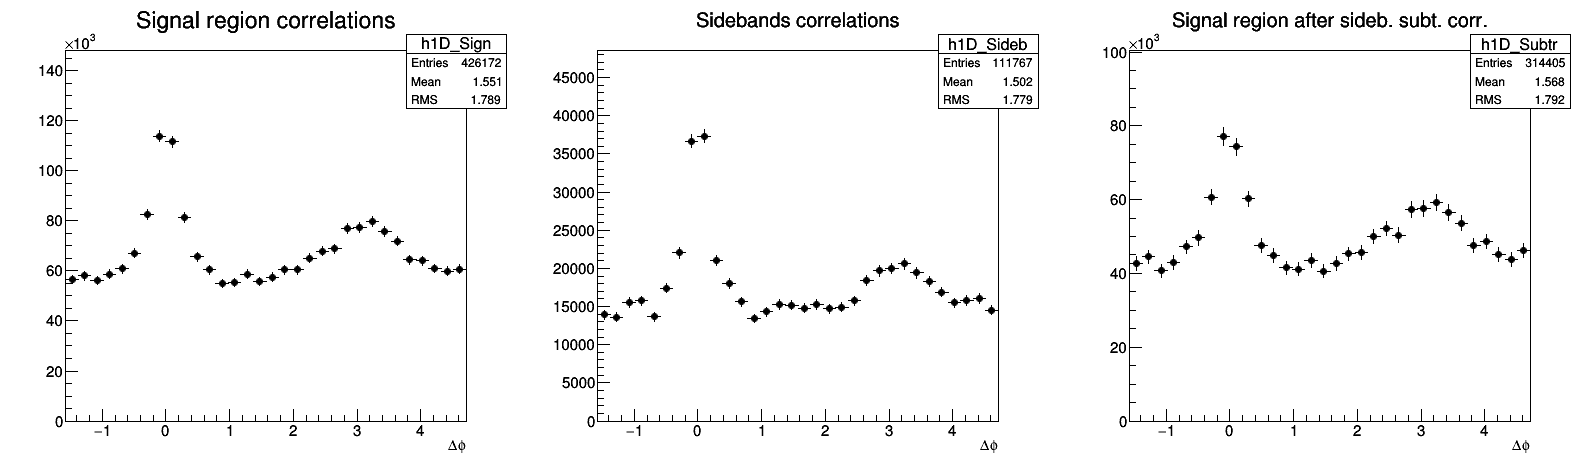
\includegraphics[width=1\linewidth]{{figures/Dzero/h1D_Dzero_Canvas_PtIntBins9to11_PoolInt_thr1dot0to99dot0.png}}
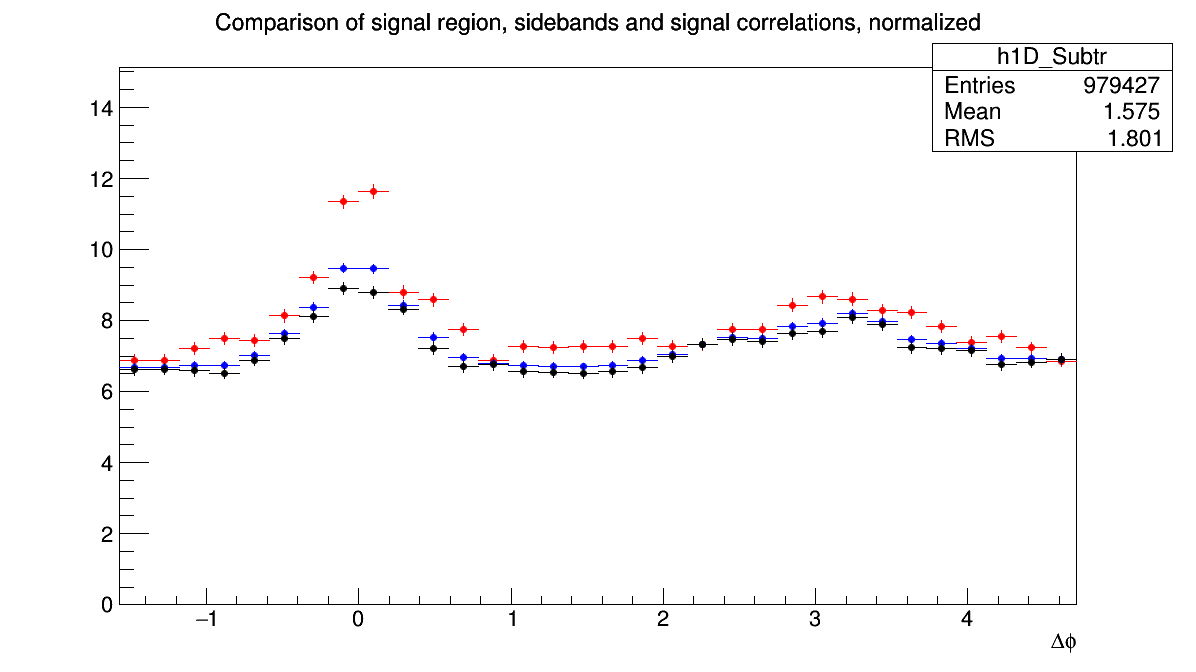
\includegraphics[width=0.8\linewidth]{{figures/Dzero/h1D_Dzero_Canvas_Normalized_PtIntBins9to11_PoolInt_thr0dot3to99dot0.png}}
\caption{Top: Example of $\Dzero$-h signal region (left), sideband (middle), and signal minus sideband (right) correlation distributions. Bottom: signal region per-trigger normalized correlation distribution (blue), sideband region per-trigger normalized correlation distribution (red),
background-subtracted per-trigger normalized correlation distribution (black).}
\label{signReg}
\end{figure}

\item
\underline{\bf Correction for D meson efficiency and associated track efficiency.}
After filling the signal and background correlation distributions, it is necessary to take into account also for the correlations with tracks, those are not reconstructed, or not passing the quality selection due to poor reconstruction. In the same way, the loss of D-mesons which are not reconstructed, or do not pass the selection, impacts the correlation distribution shape. Hence, each pair is weighted by the
inverse of the product of the associated track and D meson reconstruction efficiency, $\epsilon_{trk}$ and $\epsilon_{trig}$. Further details are provided later on in this section.

\item
\underline{\bf Projection in $\Delta\varphi$.}
The limited statistics available does not allow to study the two dimensional
$(\Delta\eta,\Delta\varphi)$ distribution, which is therefore projected to the $\Delta\varphi$ axis by integrating on $|\Delta\eta| <$ 1. Despite, in principle, our maximum $\Delta\eta$ acceptance is of $|\Delta\eta| <$ 1.6, removing the large $|\Delta\eta|$ regions allow us to reject angular regions with very low statistics, where fluctuations would be amplified by a large mixed-event correction, and avoid the so-called wings effect.

As the difference in the azimuthal angle is periodic ($\Delta \varphi = 0 = 2\pi$), the $\Delta\varphi$-range is limited to the essential range of 2$\pi$. The $\Delta \varphi$-limits are chosen to be [$-\pi$/2, 3$\pi$/2] in order to provide a good visibility of the correlation pattern, which peaks around 0 and $\pi$.

\item
\underline{\bf Correction for the contamination of secondary particles}
The DCA to primary vertex cut, applied during the associated track selection, has the role of removing the secondary particles from the associated track sample.
Secondary particles are indeed produced either from long-lived strange hadrons or from interaction of particles with the detector material. A residual contamination from secondary tracks is hence expected in the correlation distributions. This contamination is estimated from Monte Carlo simulation
based on Pythia as described more in detail in the next section. The background-subtracted
event-mixing corrected correlations are multiplied by a purity factor to encounter this contribution.

\item
\underline{\bf Correction for bias on B to D decay topologies}
The presence of the topological cuts for the D-meson selection indirecly induce a bias on the topology of the B to D decay topologies, favouring cases with a small opening angle between the D-meson and the other tracks from the B decay. This affects the feed-down component of the data correlation distributions. This effect is corrected for with a procedure described in the subsection \ref{MCclosure}. Note that this correction is a novelty with respect to the previous analyses, where only a quite conservative systematic uncertainty was applied to take into account this effect.

\item
\underline{\bf Correction for feed-down of D meson from b-hadron decay}
The selection strategy employed for the D meson candidates selection %to increase the signal over the combinatorial background
enhances the fraction of reconstructed D mesons coming from the decay of a b-hadron. Typical values, with the cuts used for the D-meson selection, are of the order of 10\% or less. The correlation distribution of these secondary D mesons will be sensitive to the properties of beauty jets and beauty hadron decay, which in general differ from those relative to charm jets and hadrons. The procedure used to subtract this contribution is described in the next paragraphs of this section.

\item
\underline{\bf Study of correlation properties.}
The properties of the azimuthal correlation distribution are quantified by
fitting the distribution with a function composed of two Gaussian functions, modelling the near and the away side peaks, and
a constant term describing the baseline. The mean of the Gaussian are fixed at
$\Delta\varphi = 0$ and $\Delta\varphi = \pi$. To accomplish the $2\pi$ periodicity
of the $\Delta\varphi$ variable, the Gaussian functions
are ``duplicated'' with mean at $\Delta\varphi = 2\pi$ and $\Delta\varphi = -\pi$.
The fitting procedure is described in details in Section \ref{results}.


%The integral of the near side peak and the away side peak
%is dominated by the central parts of the peaks at
%$\Delta \varphi = 0$ and $\Delta \varphi = \pi$, respectively. Thus, minor
%shape deviations at the side of the peak regions are  acceptable. In
%the following, the fit function is introduced step by step.
%The $\Delta \varphi$ distribution can roughly be approximated by a
%constant and two Gaussian functions with the periodicity condition.
%As the $\Delta \varphi$-distribution is a periodically continuing
%distribution with $\Delta\varphi = 0 = 2\pi$, the fit function has to
%be periodically continuing as well.

\end{enumerate}

\subsection{Mass plots and cut optimization}
The invariant mass distributions of $\Dzero$, $\Dstar$ and $\Dplus$ in the various $\text{p}_T$ ranges are shown in Figure~\ref{fig:InvMassD0},~\ref{fig:InvMassDs} and~\ref{fig:InvMassDp} respectively. Note that the distributions are weighted by the D-meson selection and reconstruction efficiency, to allow a correct normalization of the correlation distributions, which have also these weights.

\begin{figure}[!htp]
\centering

{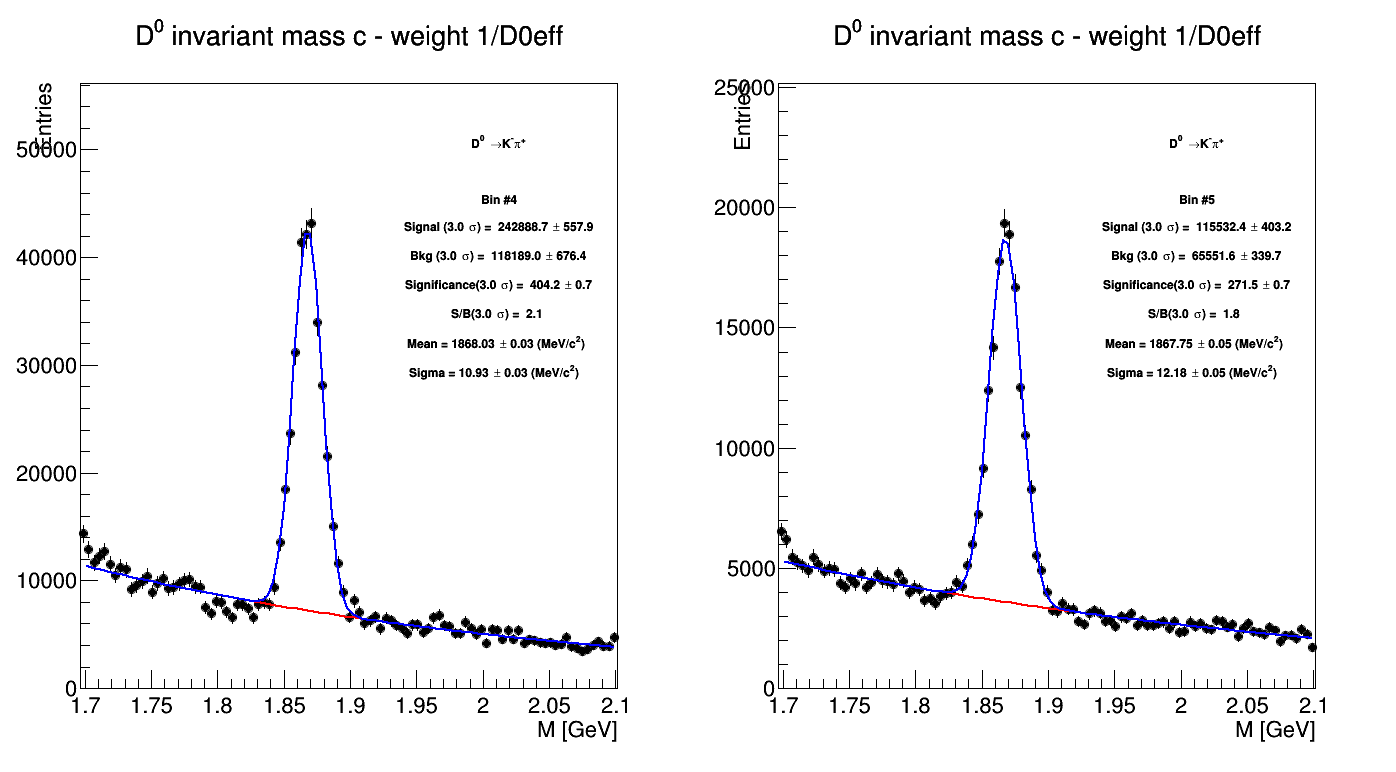
\includegraphics[width=1\linewidth, height=5.6cm]{figures/Dzero/InvMassDistributions_Dzero_Bins4to5.png}}
{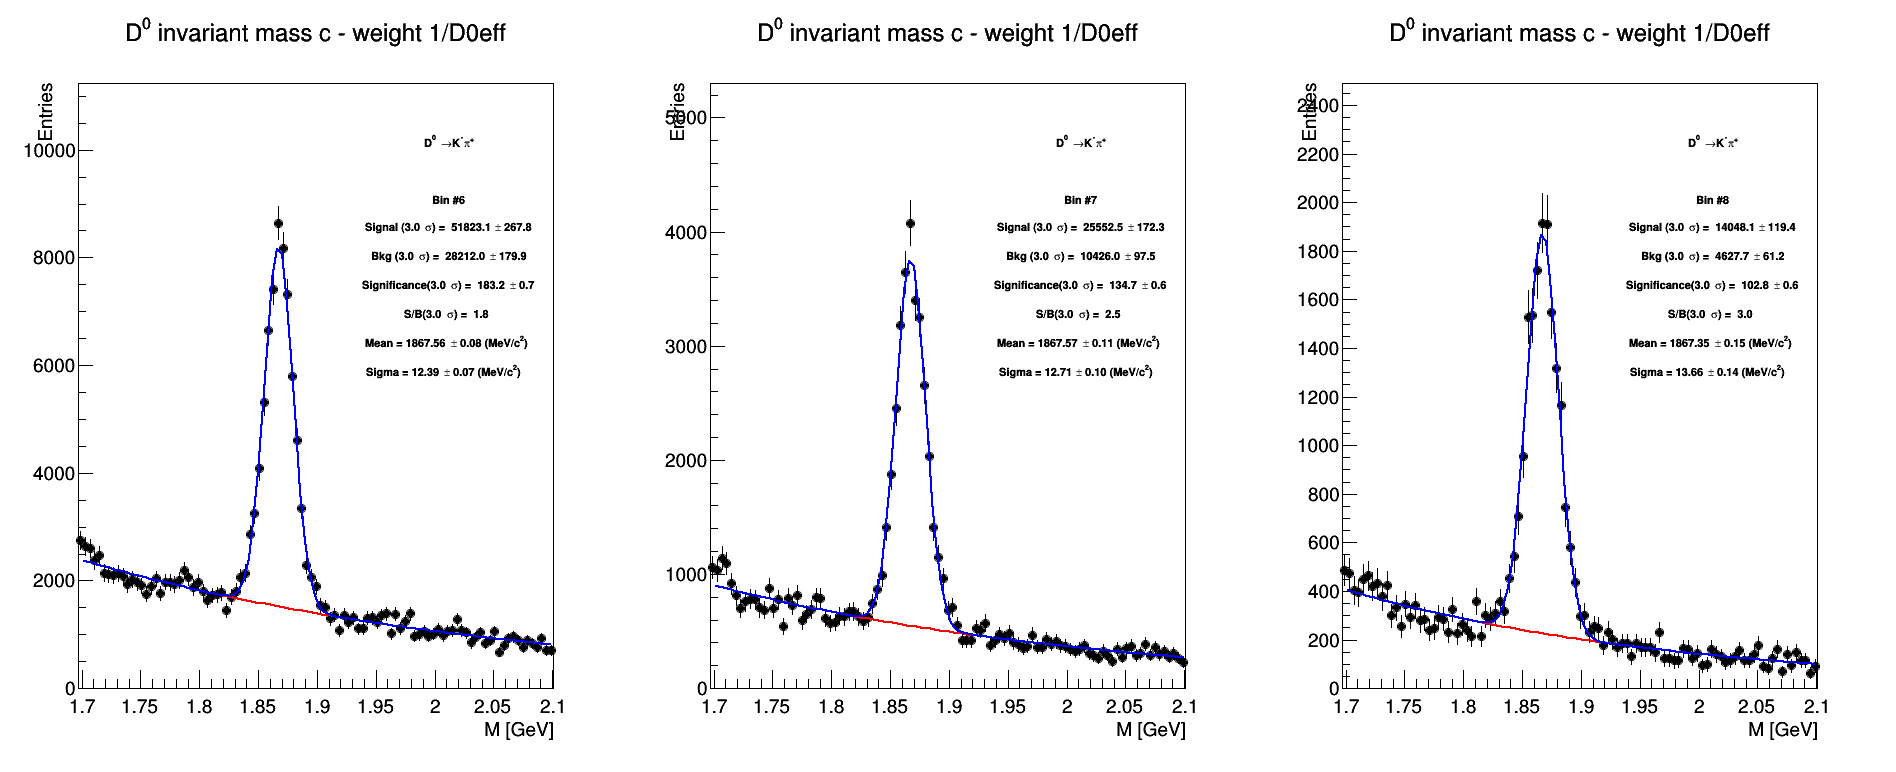
\includegraphics[width=1\linewidth, height=5.6cm]{figures/Dzero/InvMassDistributions_Dzero_Bins6to8.png}}
{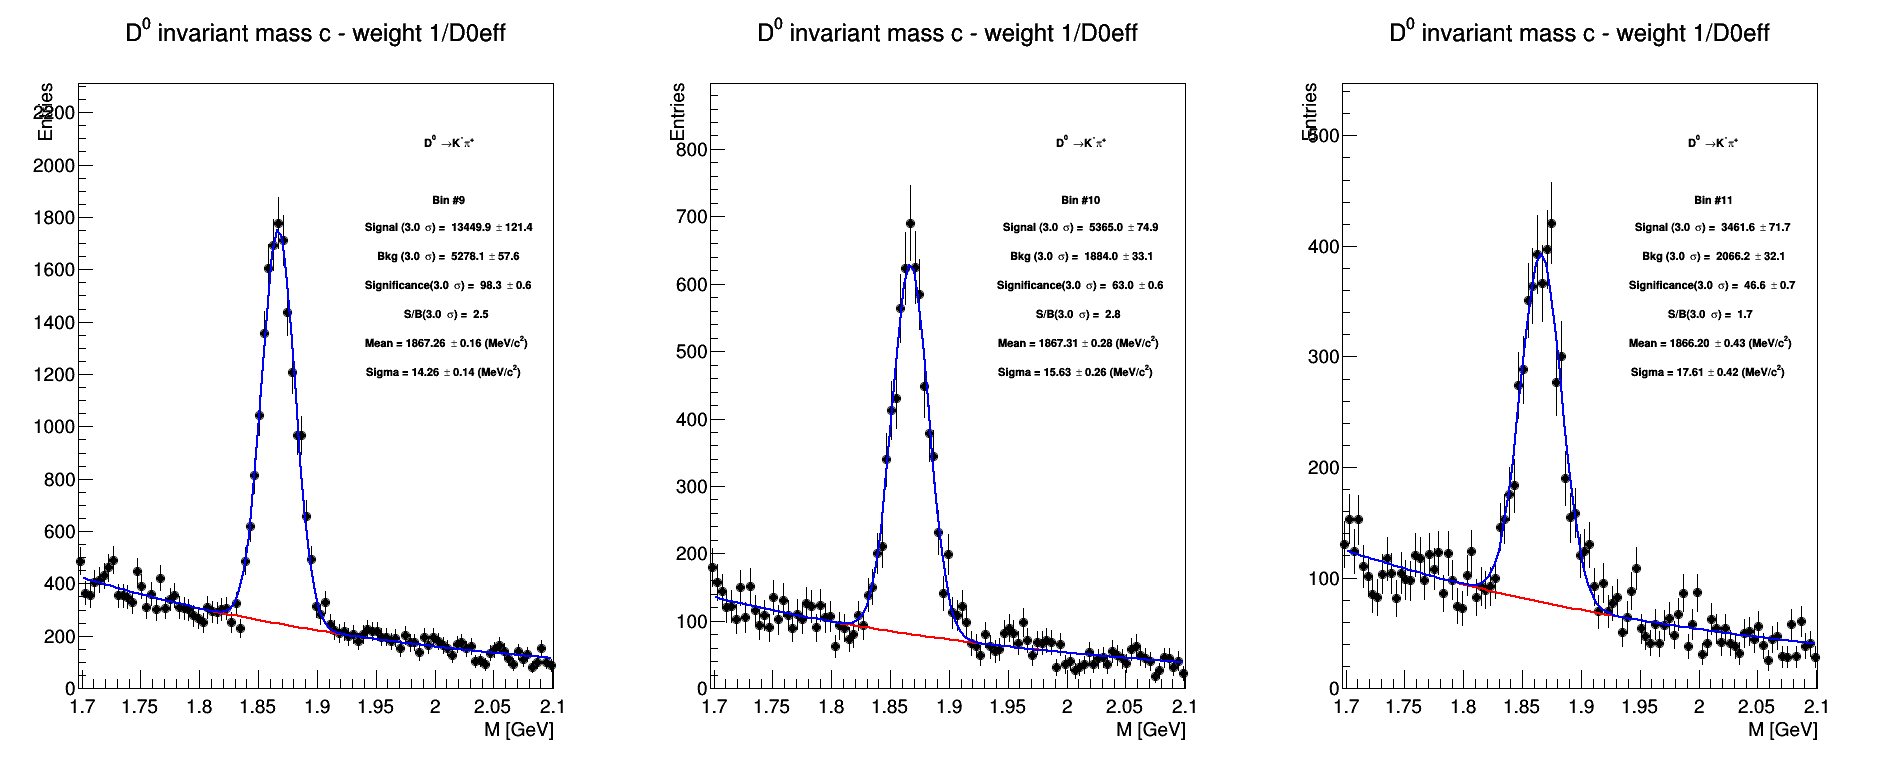
\includegraphics[width=1\linewidth, height=5.6cm]{figures/Dzero/InvMassDistributions_Dzero_Bins9to11.png}}
{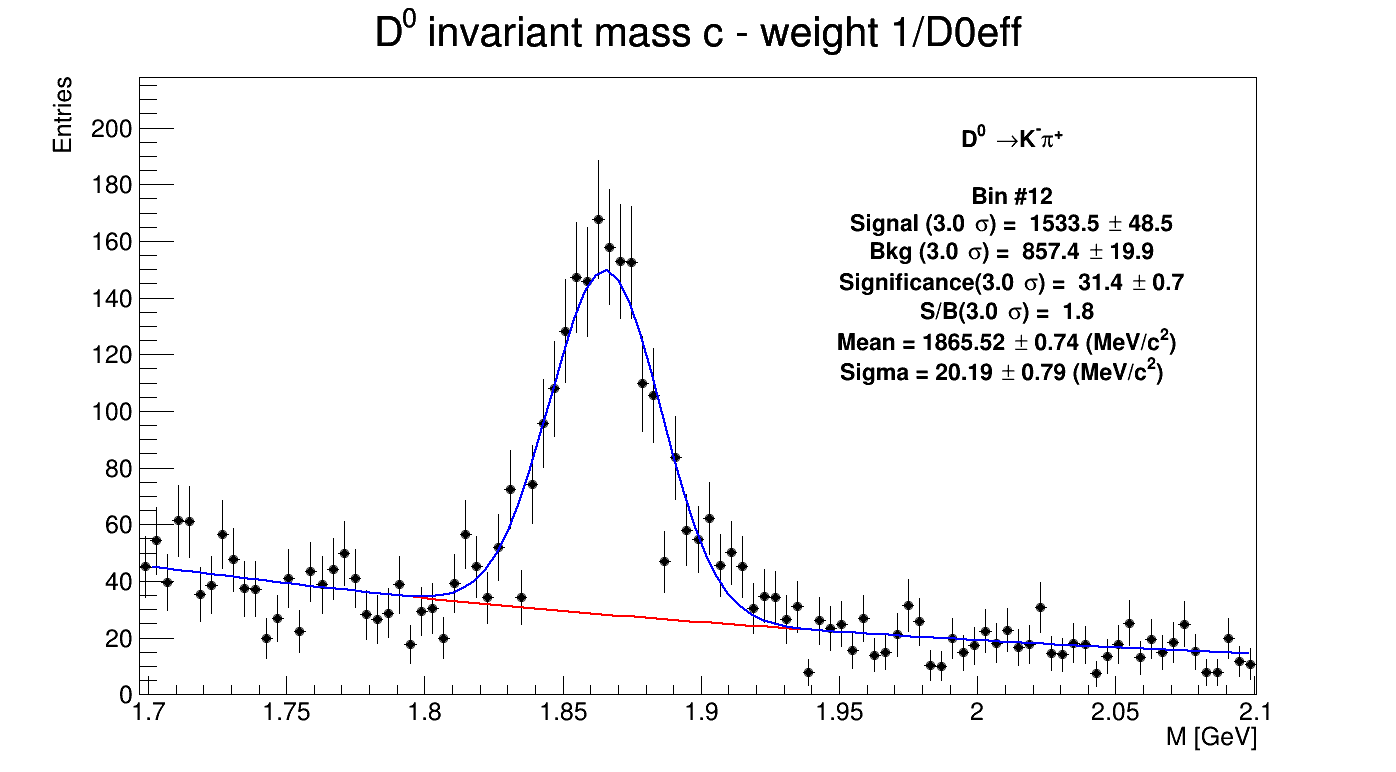
\includegraphics[width=0.6\linewidth, height=5.6cm]{figures/Dzero/InvMassDistributions_Dzero_Bins12to12.png}}

%[width=.32\linewidth]
\caption{Invariant mass distributions of $D^0$ corrected with efficiency in different $\text{p}_T$ regions. Top: $3< p_{T}^{\text{D}}< 4$ $\gev/c$ (left), $4< p_{T}^{\text{D}}< 5$ $\gev/c$ right), Mid 1: $5< p_{T}^{\text{D}}< 6$ $\gev/c$ (left), $6 < p_{T}^{\text{D}} < 7$ $\gev/c$ (middle), $7< p_{T}^{\text{D}}< 8$ $\gev/c$ (right); Mid2: $8< p_{T}^{\text{D}}< 10$ $\gev/c$, $10< p_{T}^{\text{D}}< 12$ $\gev/c$  (middle), $12 < p_{T}^{\text{D}}< 16$ $\gev/c$  (right) and Bottom: $16<p_{T}^{\text{D}}< 24$ $\gev/c$.}
\label{fig:InvMassD0}
\end{figure}

\begin{figure}[!htp]
\centering
{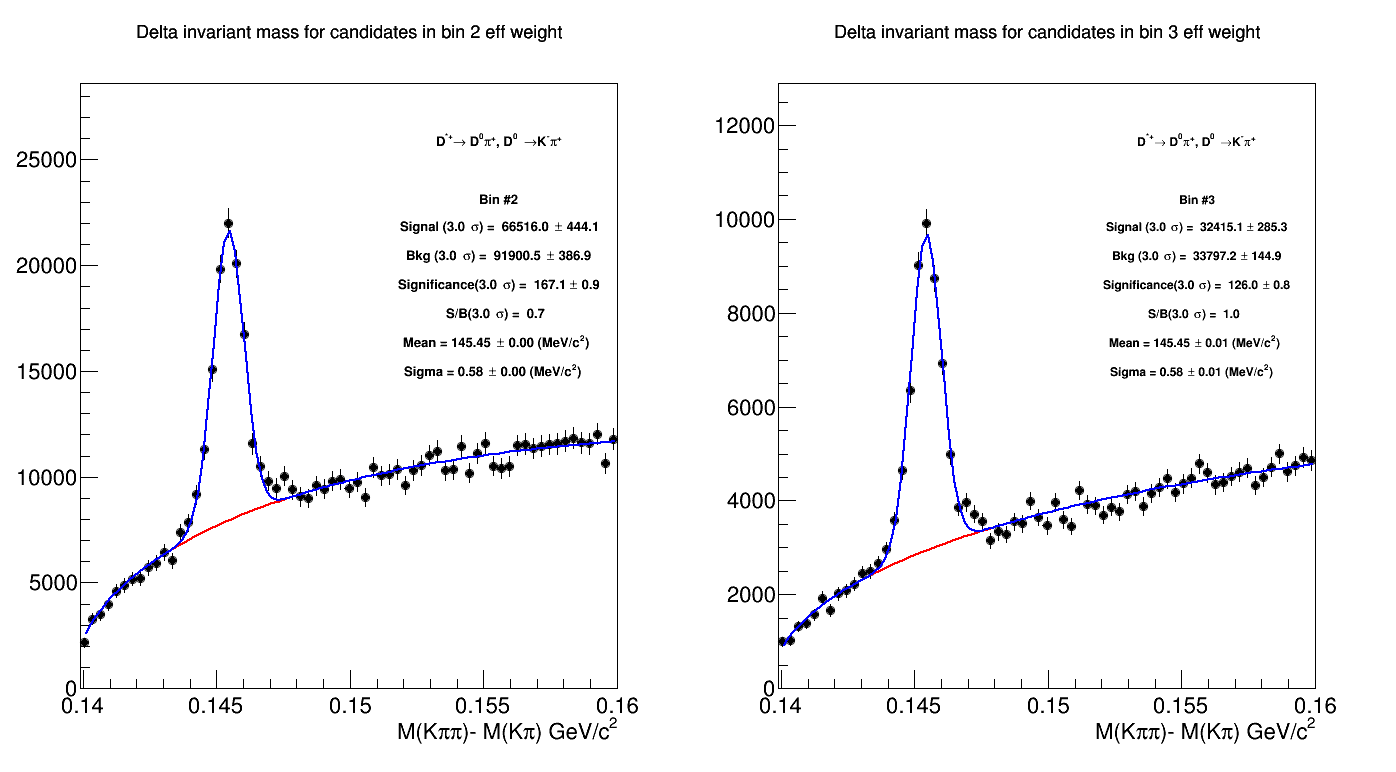
\includegraphics[width=1\linewidth, height=5.6cm]{figures/Dstar_wEFF/InvMassDistributions_Dstar_Bins2to3.png}}
{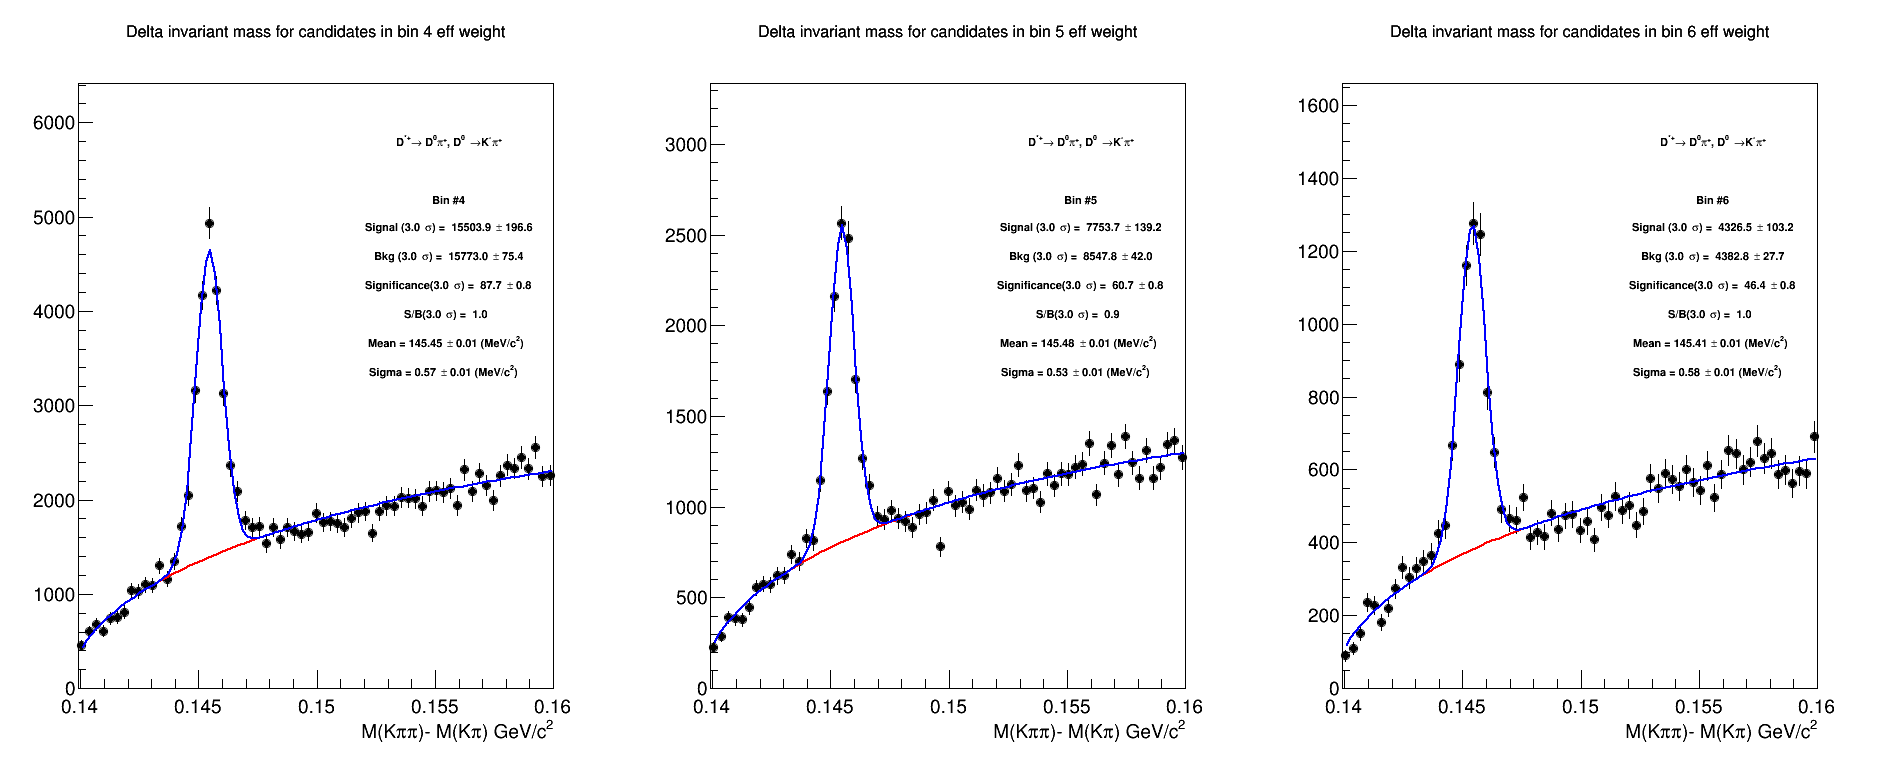
\includegraphics[width=1\linewidth, height=5.6cm]{figures/Dstar_wEFF/InvMassDistributions_Dstar_Bins4to6.png}}
{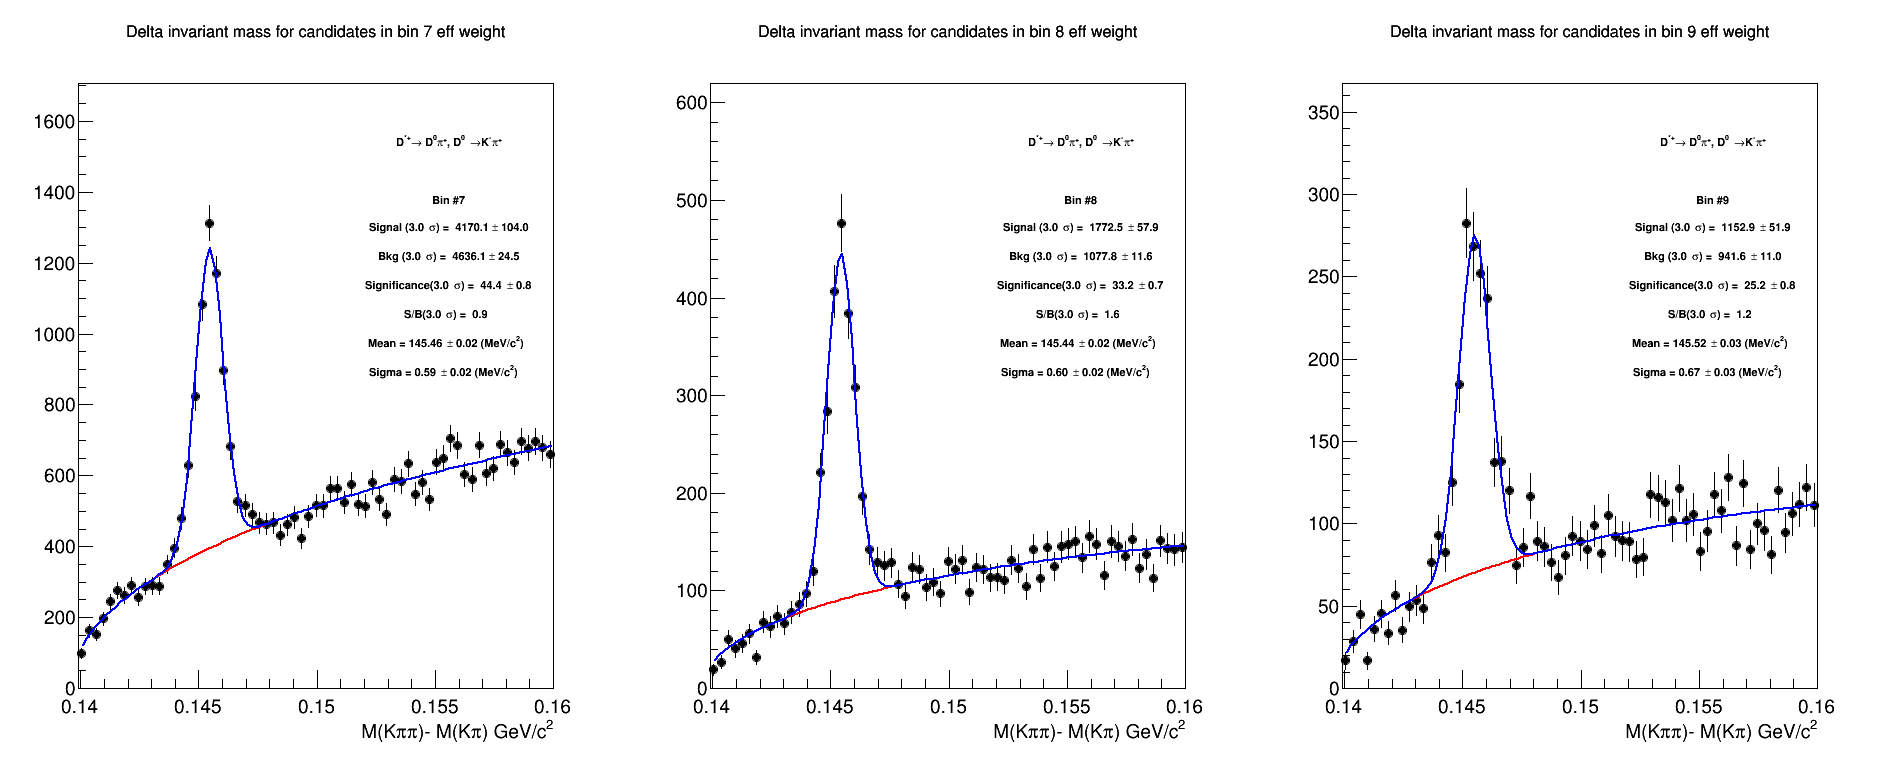
\includegraphics[width=1\linewidth, height=5.6cm]{figures/Dstar_wEFF/InvMassDistributions_Dstar_Bins7to9.png}}
{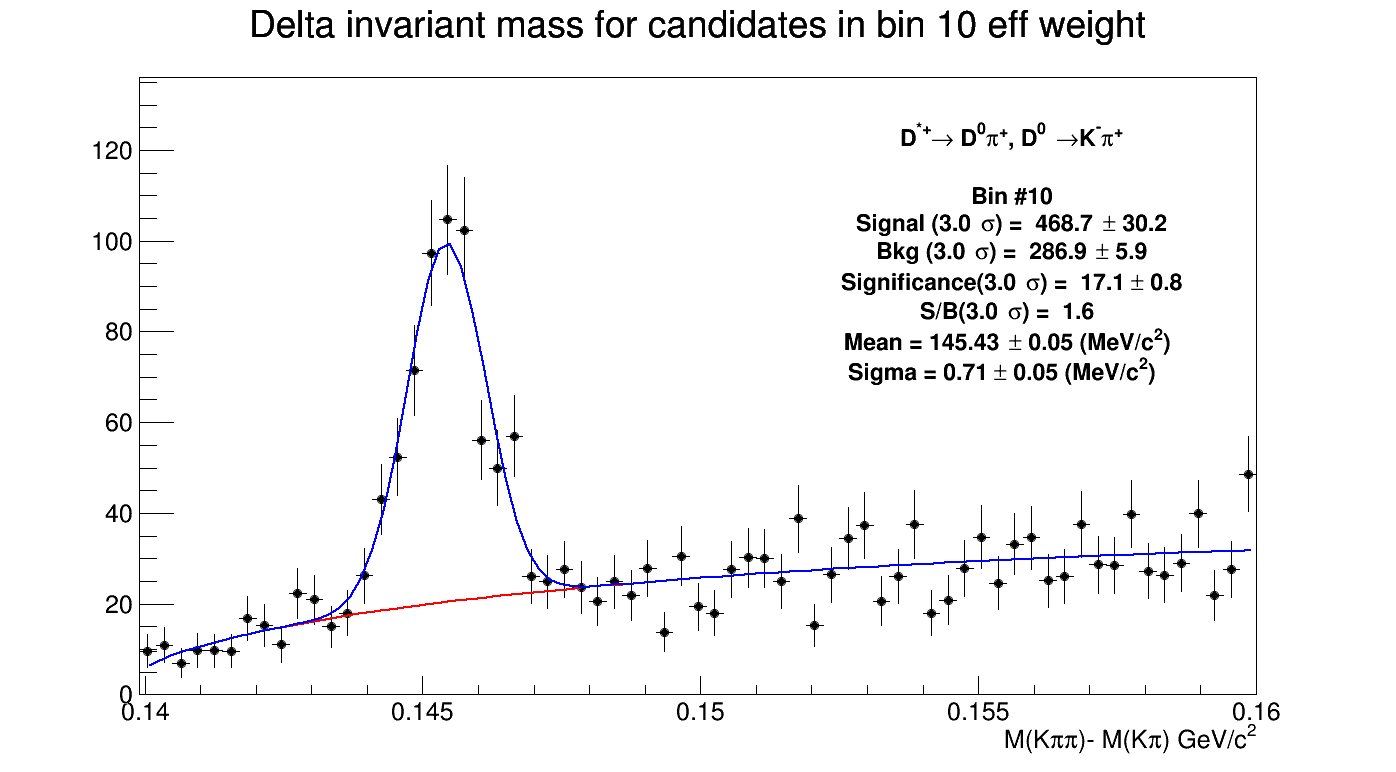
\includegraphics[width=0.6\linewidth, height=5.6cm]{figures/Dstar_wEFF/InvMassDistributions_Dstar_Bins10to10.png}}

\caption{Invariant mass distributions of $\Dstar$ corrected with efficiency in different $\text{p}_T$ regions. Top: $3< p_{T}^{\text{D}}< 4$ $\gev/c$ (left), $4< p_{T}^{\text{D}}< 5$ $\gev/c$ right), Mid 1: $5< p_{T}^{\text{D}}< 6$ $\gev/c$ (left), $6 < p_{T}^{\text{D}} < 7$ $\gev/c$ (middle), $7< p_{T}^{\text{D}}< 8$ $\gev/c$ (right); Mid2: $8< p_{T}^{\text{D}}< 10$ $\gev/c$, $10< p_{T}^{\text{D}}< 12$ $\gev/c$  (middle), $12 < p_{T}^{\text{D}}< 16$ $\gev/c$  (right) and Bottom: $16<p_{T}^{\text{D}}< 24$ $\gev/c$ .}
\label{fig:InvMassDs}
\end{figure}

\begin{figure}[!htp]
\centering
{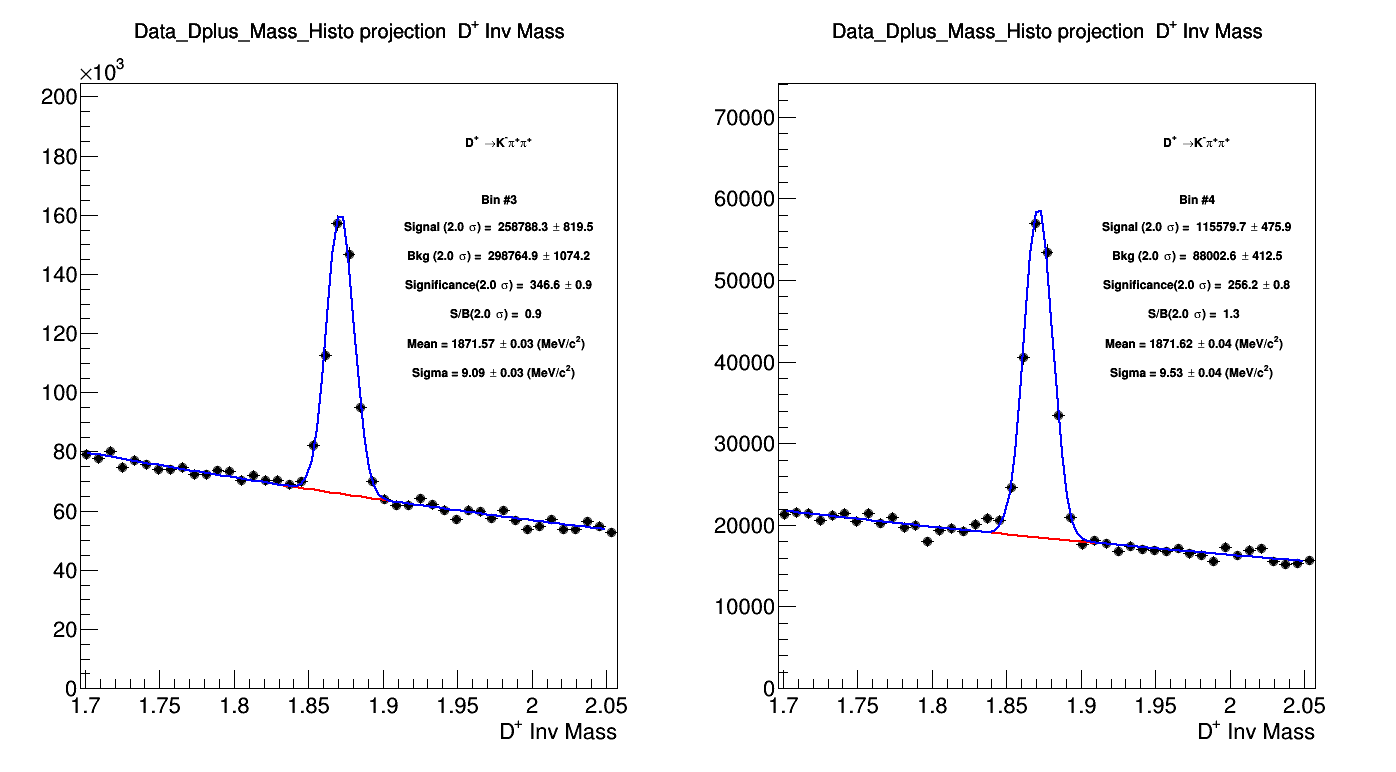
\includegraphics[width=1\linewidth, height=5.6cm]{figures/DplusPlotsweff/InvMassDistributions_Dplus_Bins3to4.png}}
{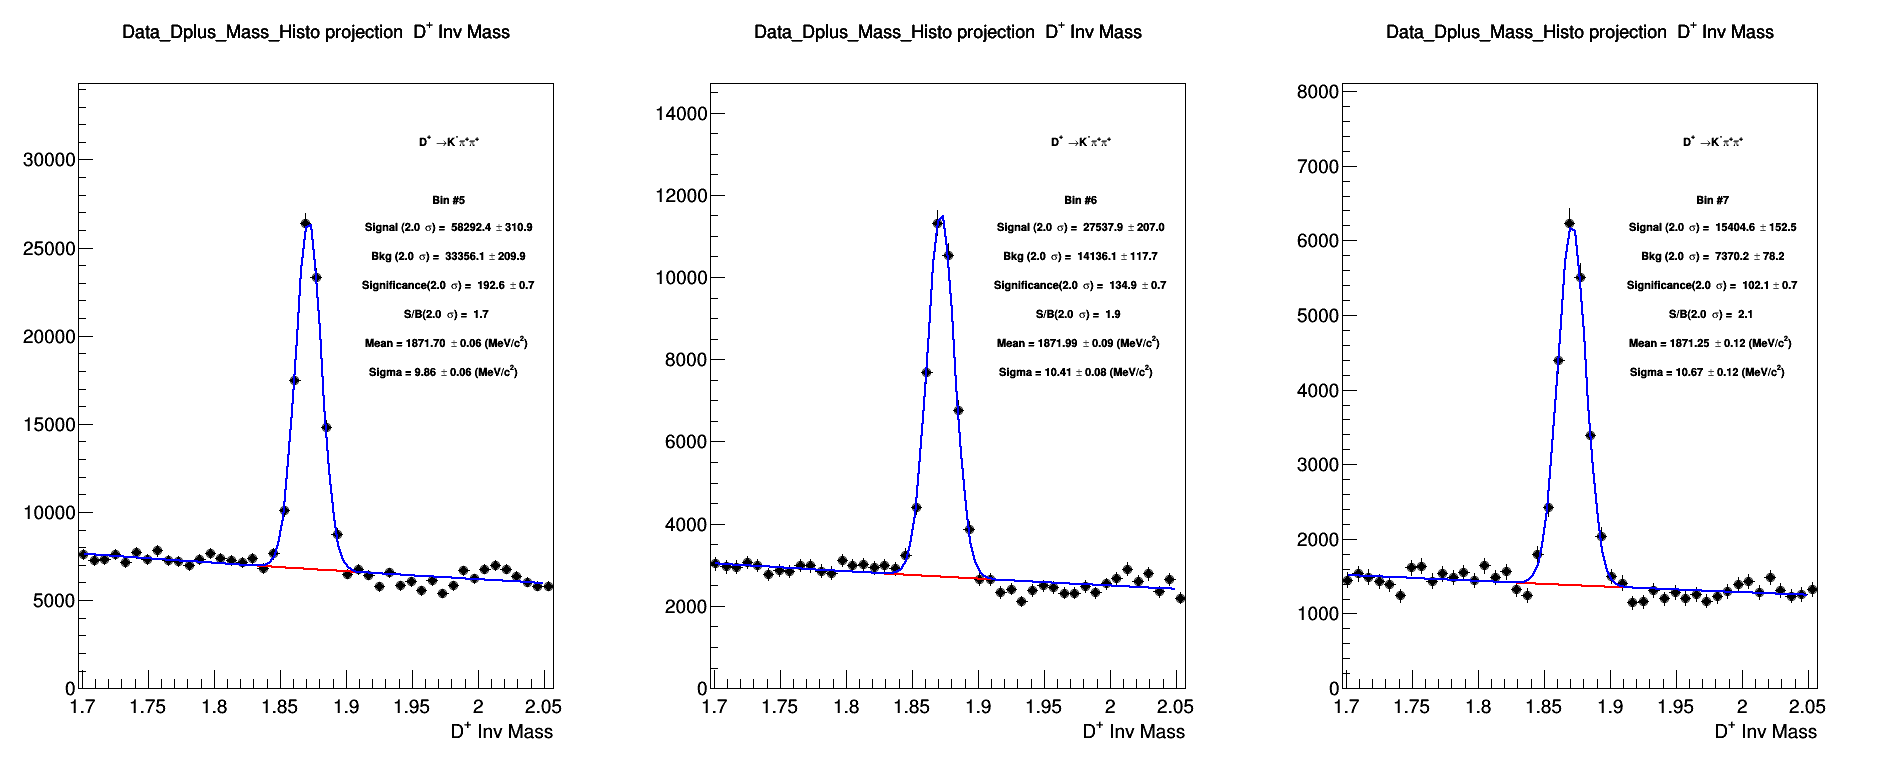
\includegraphics[width=1\linewidth, height=5.6cm]{figures/DplusPlotsweff/InvMassDistributions_Dplus_Bins5to7.png}}
{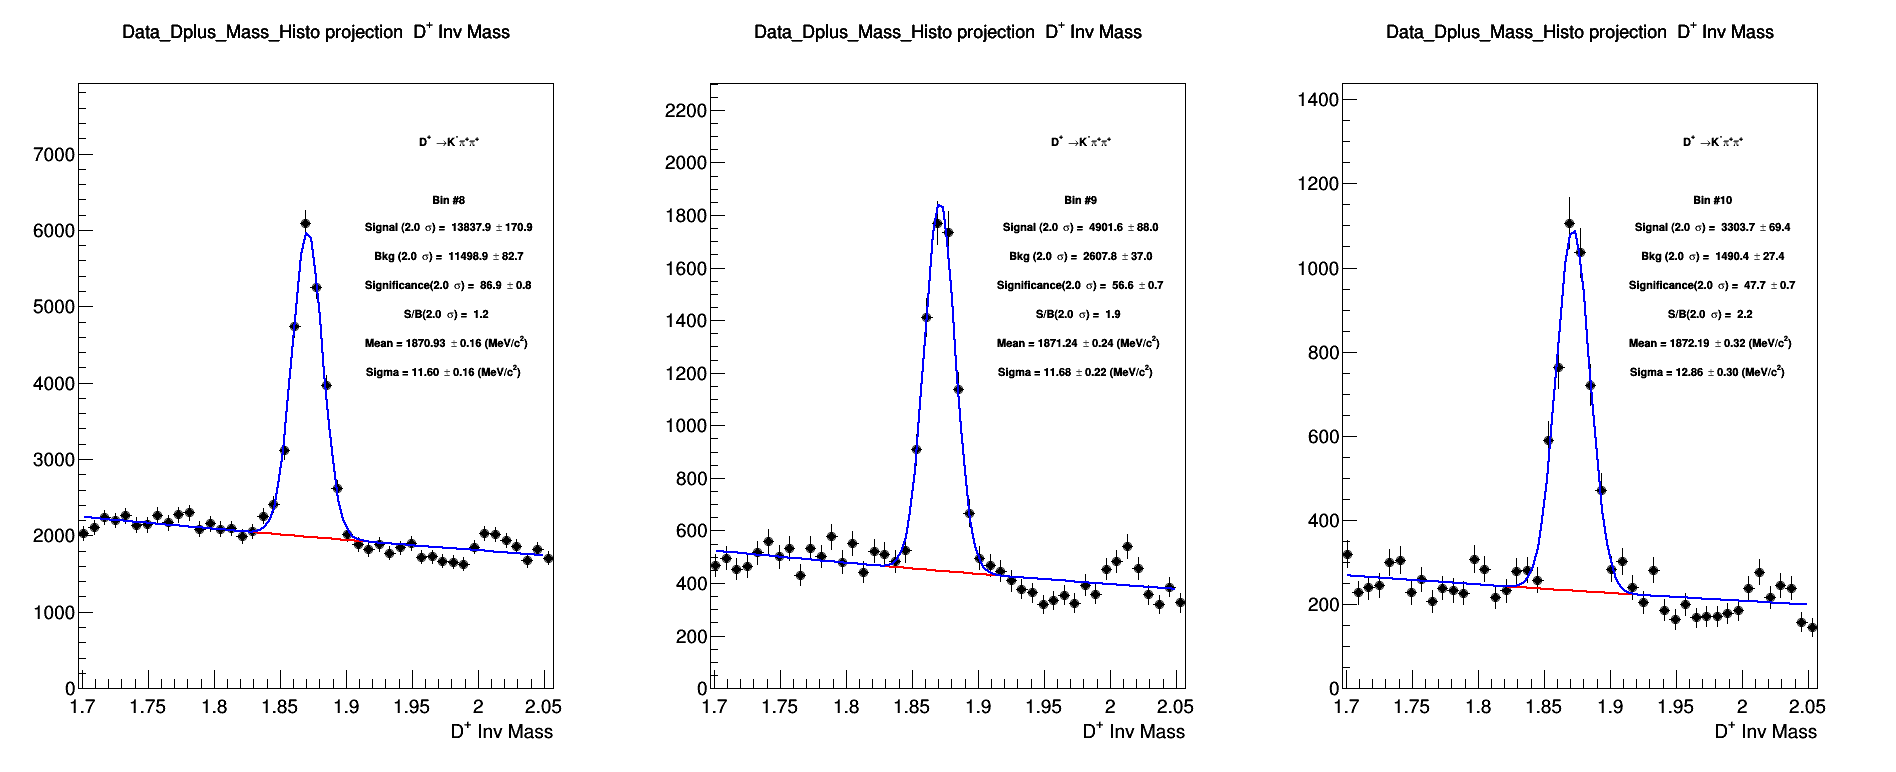
\includegraphics[width=1\linewidth, height=5.6cm]{figures/DplusPlotsweff/InvMassDistributions_Dplus_Bins8to10.png}}
{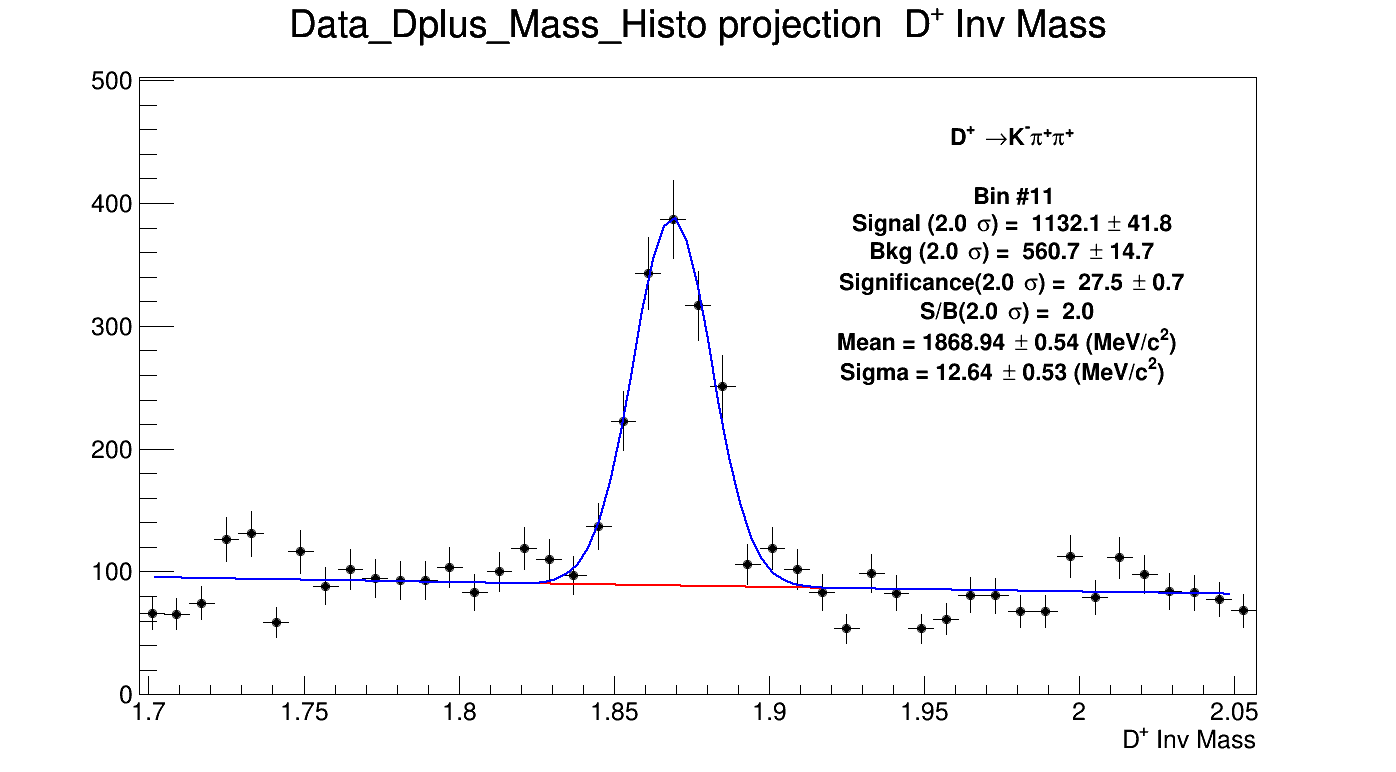
\includegraphics[width=0.6\linewidth, height=5.6cm]{figures/DplusPlotsweff/InvMassDistributions_Dplus_Bins11to11.png}}

\caption{Invariant mass distribution of $\Dplus$ corrected with efficiency in different $\text{p}_T$ regions. Top: $3< p_{T}^{\text{D}}< 4$ $\gev/c$ (left), $4< p_{T}^{\text{D}}< 5$ $\gev/c$ right), Mid 1: $5< p_{T}^{\text{D}}< 6$ $\gev/c$ (left), $6 < p_{T}^{\text{D}} < 7$ $\gev/c$ (middle), $7< p_{T}^{\text{D}}< 8$ $\gev/c$ (right); Mid2: $8< p_{T}^{\text{D}}< 10$ $\gev/c$, $10< p_{T}^{\text{D}}< 12$ $\gev/c$  (middle), $12 < p_{T}^{\text{D}}< 16$ $\gev/c$  (right) and Bottom: $16<p_{T}^{\text{D}}< 24$ $\gev/c$ .}
\label{fig:InvMassDp}
\end{figure}

For $\Dstar$, the standard D2H p-Pb cuts (for the 2013 cross section analysis, \cite{NoteD2HpPb}) were used. The same holds for the $\Dplus$, but with the addition of cuts on the normalized decay length in $xy$ plane and of the normalized difference between measured and expected daughter track impact parameters (topomatic cut).
A particular cut optimization was instead performed for the $\Dzero$ meson. Twelve cut sets were tried, with the goal of increasing the S/B factor, in order to reduce fluctuations induced by the sideband subraction (the limiting factor for the analysis performance).
In Figure \ref{fig:cutoptD0} the $\Dzero$-h correlation distributions are shown for the different cut sets, in exemplary kinematic regions (left column), together with the bin-by-bin relative statistical uncertainty on the data points (right column). The best cut set (option G) was defined from the standard cuts used for the p-Pb 2013 cross section analysis, with a tightened selection on the cosine of the pointing angle, and with the addition of a cut on the normalized decay length in $xy$ plane and of a selection on the normalized difference between measured and expected daughter track impact parameters (topomatic cut).

\begin{figure}[!htp]
\centering
{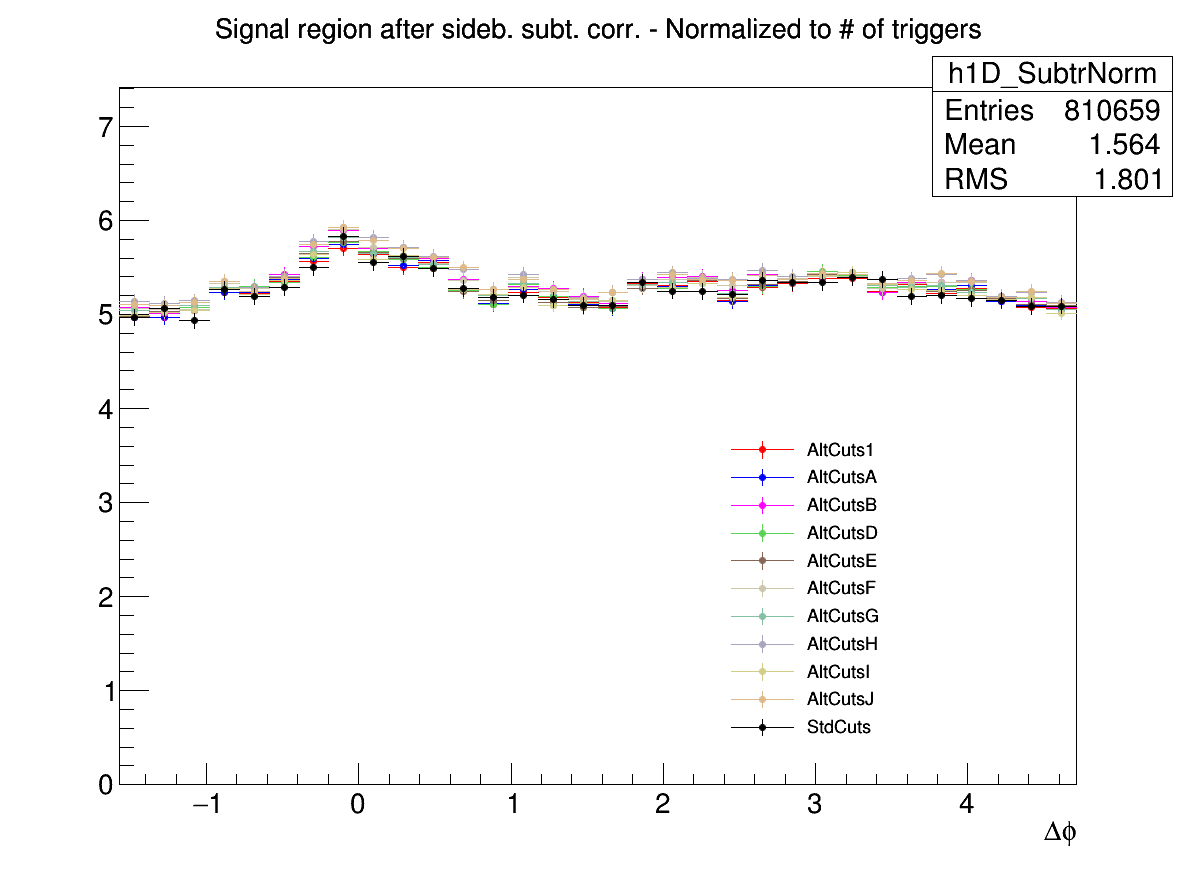
\includegraphics[width=0.47\linewidth, height=5.6cm]{figures/Cut_Optimiz_D0/AzimCorrDistr_Dzero_Canvas_PtIntBins3to5_PoolInt_thr03to99_Superimp.png}}
{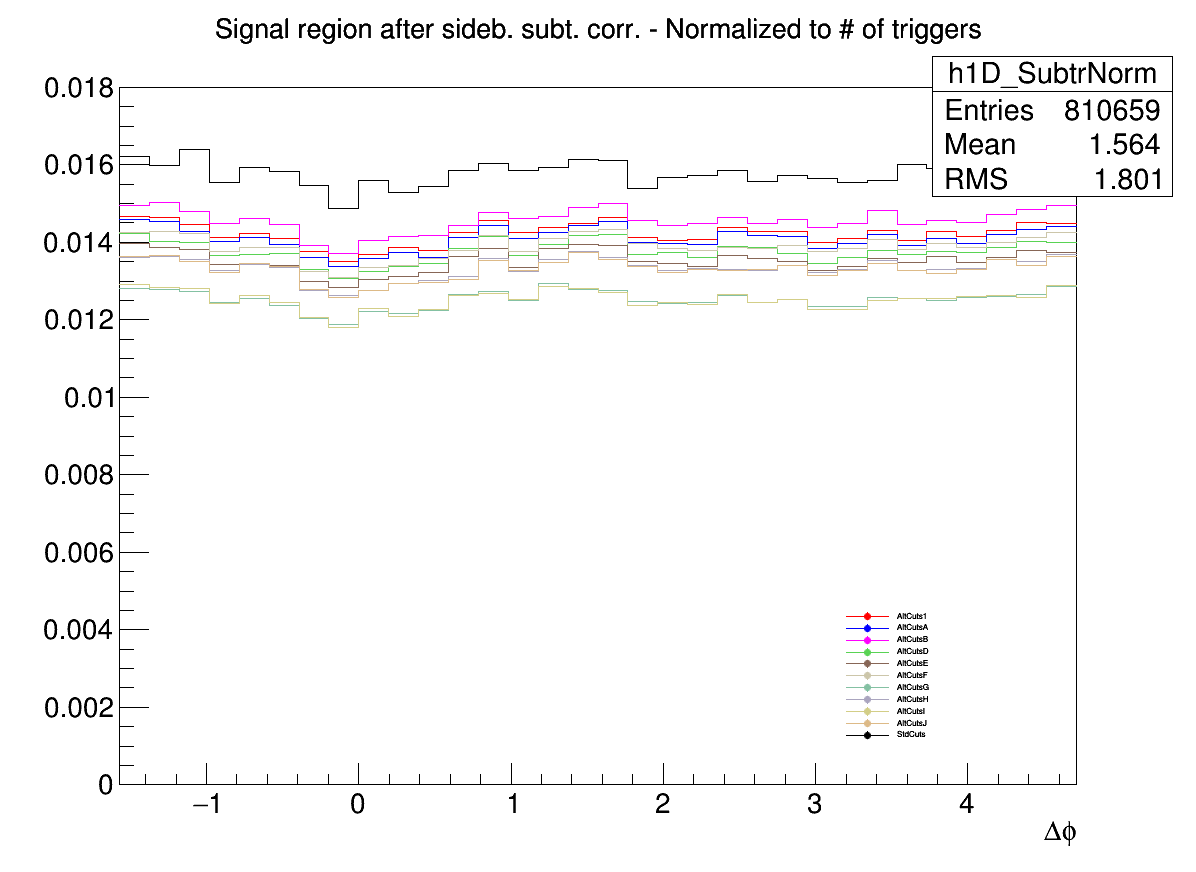
\includegraphics[width=0.47\linewidth, height=5.6cm]{figures/Cut_Optimiz_D0/Uncertanty_AzimCorrDistr_Dzero_Canvas_PtIntBins3to5_PoolInt_thr03to99.png}}
{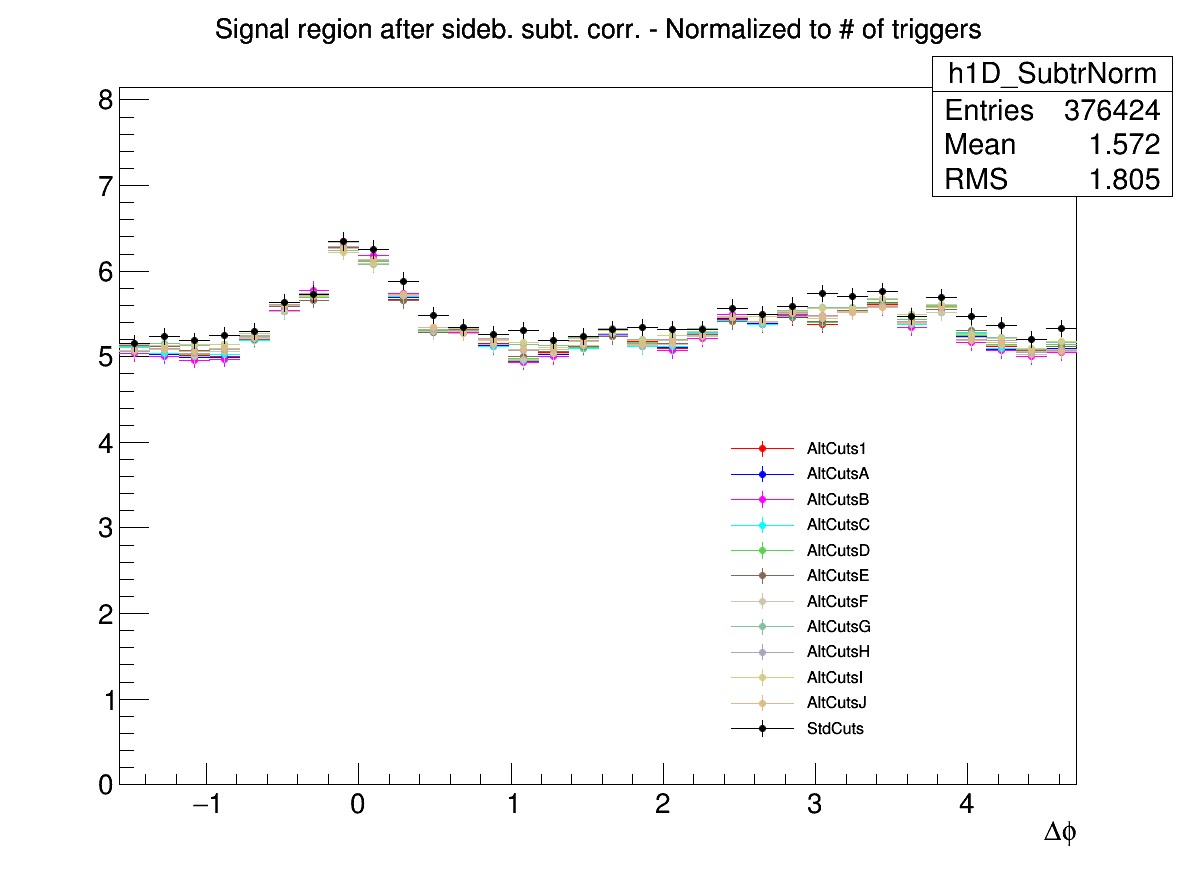
\includegraphics[width=0.47\linewidth, height=5.6cm]{figures/Cut_Optimiz_D0/AzimCorrDistr_Dzero_Canvas_PtIntBins6to8_PoolInt_thr03to99_Superimp.png}}
{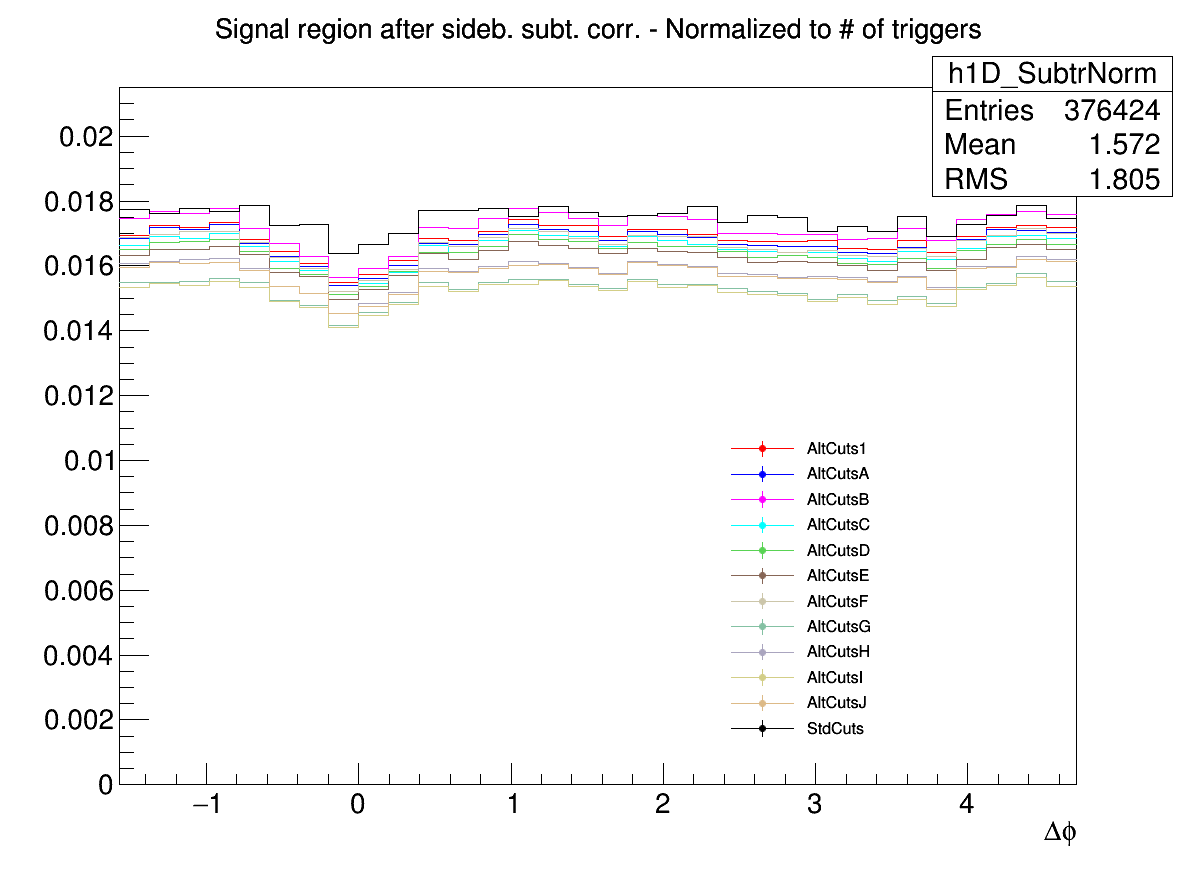
\includegraphics[width=0.47\linewidth, height=5.6cm]{figures/Cut_Optimiz_D0/Uncertanty_AzimCorrDistr_Dzero_Canvas_PtIntBins6to8_PoolInt_thr03to99.png}}
{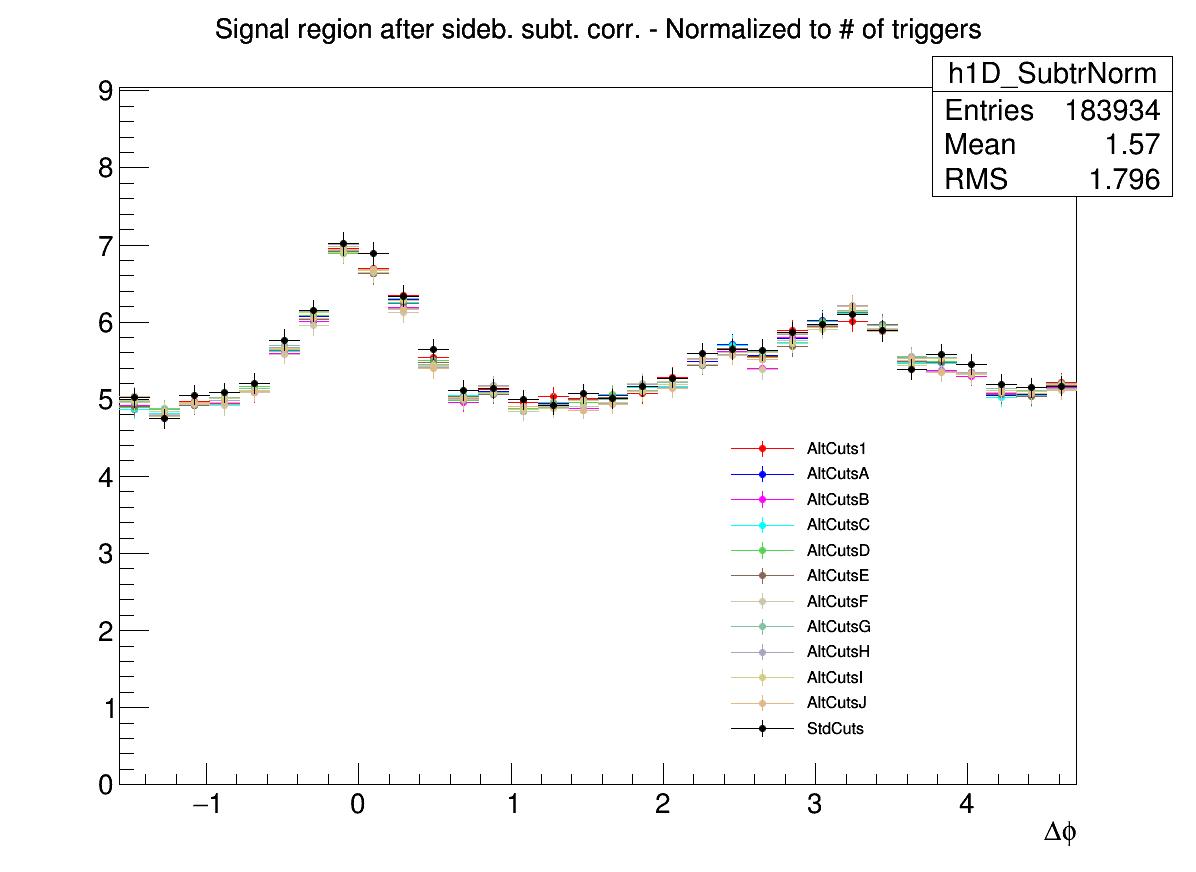
\includegraphics[width=0.47\linewidth, height=5.6cm]{figures/Cut_Optimiz_D0/AzimCorrDistr_Dzero_Canvas_PtIntBins9to10_PoolInt_thr03to99_Superimp.png}}
{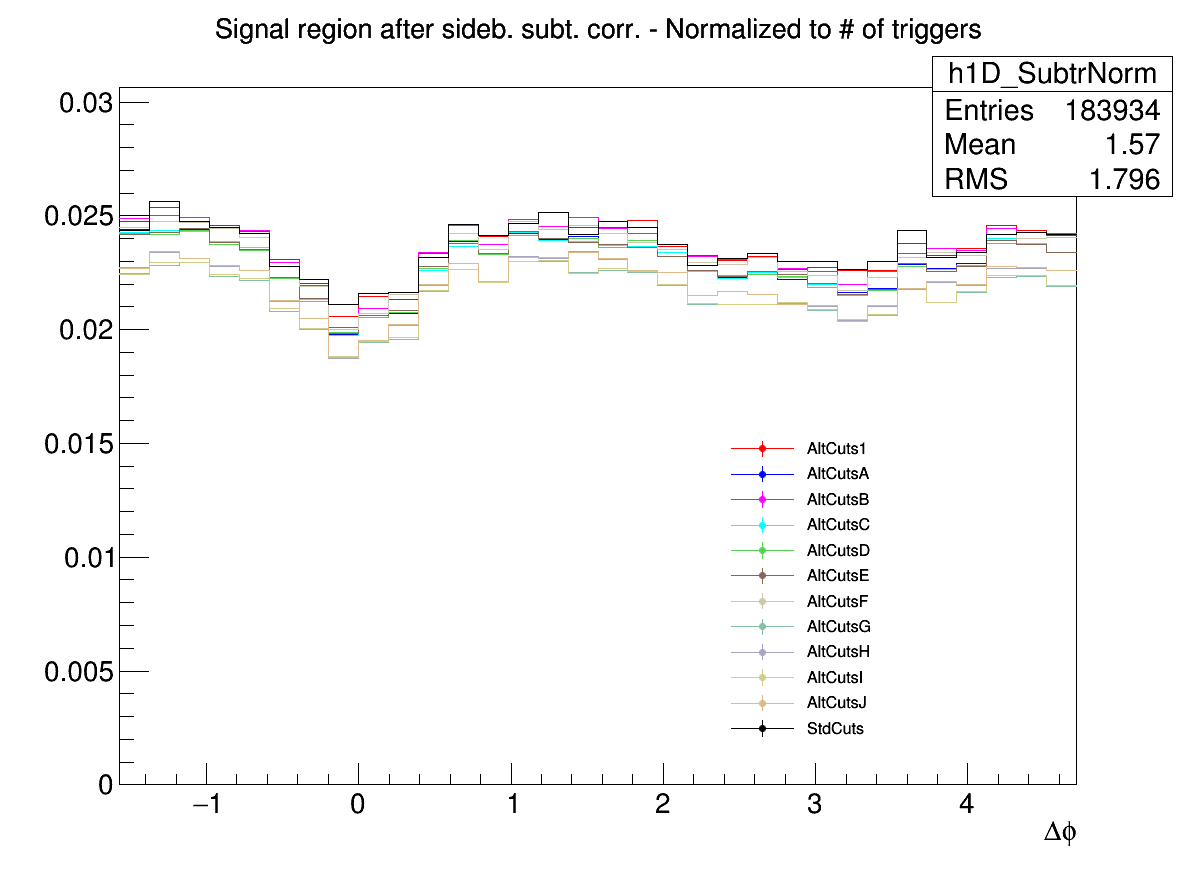
\includegraphics[width=0.47\linewidth, height=5.6cm]{figures/Cut_Optimiz_D0/Uncertanty_AzimCorrDistr_Dzero_Canvas_PtIntBins9to10_PoolInt_thr03to99.png}}

\caption{$\Dzero$-h correlation distributions with different cut options (left) and point-by-point relative statistical uncertainty (right) for $3< p_{T}^{\text{D}}< 5$ $\gev/c$ (top), $5< p_{T}^{\text{D}}< 8$ $\gev/c$ (middle), $8< p_{T}^{\text{D}}< 16$ $\gev/c$ (bottom), in all cases with associated track $\pt$ $> 0.3$ $\gev/c$.}
\label{fig:cutoptD0}
\end{figure}

\subsection{Code used for the analysis}
The code used for D meson-hadron correlation analysis is fully committed in AliPhysics. The analysis classes can be found in
\$ALICE\_ROOT/PWGHF/correlationHF/.  The  D meson specific classes where the aforementioned steps are carried out are
AliAnalysisTaskDStarCorrelations, AliAnalysisTaskSED0Correlations and AliAnalysisTaskDplusCorrelations. The classes which are common to the D meson specific analysis which includes the associated particle cuts and the correlation observables are AliHFAssociatedTrackCuts, AliHFCorrelator, AliHFOfflineCorrelator, AliReducedParticle and AliDhCorrelationExtraction. Several additional classes and macros in the same folder deal with the correction steps.

The final results presented here are extracted are the HFCJ pPb (n. 88) train runs 290-293 (for $\Dzero$ and $\Dplus$) and 286-289 (for $\Dstar$).

\subsection{Further details on corrections}
\subsubsection{Event Mixing}
\input{./Sections/3Analysis_Strategy/EventMixing.tex}

\begin{comment}
\begin{figure}[!ht]
\centering
%{\includegraphics[width=.95\linewidth]{figures/Dplus_low_dot5_SEbyME.png}}
 \caption{($\Delta \varphi , \Delta \eta$) correlation in the Sidebands and Signal region from Single Event and Mixing Event analysis for low $p_{T}$: $3 < p_{T}^{\text{D}^+} < 5 $\gev/c$$ with associated track $p_{T}$ threshold 0.3 $\gev/c$ }
\label{fig:DplusSEbyMEPlots1}
\end{figure}



\begin{figure}[!ht]
\centering
%Marianna
%{\includegraphics[width=.95\linewidth]{figures/Dplus_mid_dot5_SEbyME.png}}
 \caption{($\Delta \varphi , \Delta \eta$) correlation in the Sidebands and Signal region from Single Event and Mixing Event analysis for mid $p_{T}$: $5< p_{T}^{\text{D}^+}< 8 $\gev/c$$ with associated track $p_{T}$ threshold 0.3 $\gev/c$ }
\label{fig:DplusSEbyMEPlots2}
\end{figure}

\begin{figure}[!ht]
\centering
%{\includegraphics[width=.95\linewidth]{figures/Dplus_high_dot5_SEbyME.png}}
 \caption{($\Delta \varphi , \Delta \eta$) correlation in the Sidebands and Signal region from Single Event and Mixing Event analysis for high $p_{T}$: $8< p_{T}^{\text{D}^+}< 16 $\gev/c$$ with associcated track $p_{T}$ threshold 0.3 $\gev/c$ }
\label{fig:DplusSEbyMEPlots3}
\end{figure}

Figures \ref{fig:DplusSEbyMEPlots1}, \ref{fig:DplusSEbyMEPlots2}, \ref{fig:DplusSEbyMEPlots3} show the 2D correlation in Sideband Region and Signal region from SE and ME analysis for $D^+$ meson in different $p_{T}$ region.

\end{comment}

\newpage
\subsubsection{Tracking and D-meson trigger efficiency}
{\bf \normalsize (i) Tracking efficiency} - The tracking efficiency was calculated by obtaining the ratio between the yield at the reconstructed level and generated level, for a defined ``type" of particles (in our case non-identified particles) and it is estimated differentially in p$_T$, $\eta$, and z$_{vtx}$ of the charged particles.\\

Tracking efficiency maps were produced as TH3D histograms (p$_T$, $\eta$, z$_{vtx}$) obtained from MC analysis on the minimum-bias samples LHC17f2b$\_$fast and LHC17f2b$\_$cent$\_$woSDD, considering only primary pions, kaons, protons, electrons and muons, and applying at reconstructed level the track selections (summarized in Table.~\ref{table:effCuts}). These efficiency maps were used in the analysis tasks to extract single track efficiencies; each correlation pairs found in the data analysis was inserted in correlation plots with a weight of {\bf 1/efficiency value}. 
As a cross-check, the tracking efficiency was evaluated, with the same criteria, also on the LHC17f2a$\_$fast and LHC17f2a$\_$cent$\_$woSDD samples, which were produced with EPOS-LHC generator instead of DPMJET. Compatibility within 1\% between the efficiency values on the two samples was found.
The 1D ($\pt$ dependence) tracking efficiency, evaluated on f2b samples (blue) and on f2a samples (red) are shown in Fig.~\ref{fig:trackeff}, as well as the ratio of f2b over f2a efficiencies.

\begin{figure}[h]
	\centering
	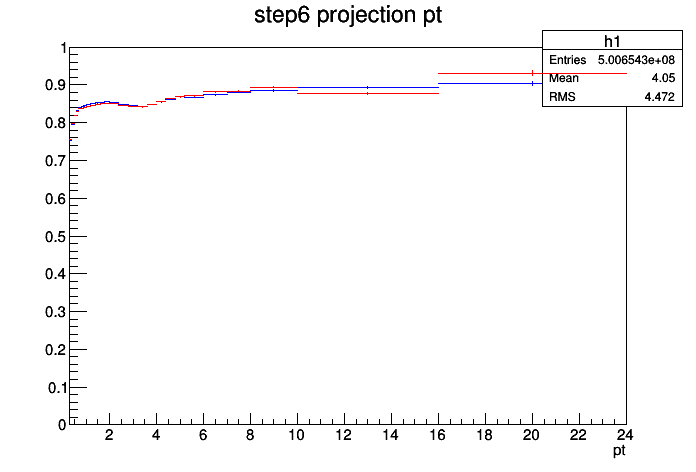
\includegraphics[width=0.8\linewidth]{figures/Effs/CompareEff_FiveSpecies.png}
    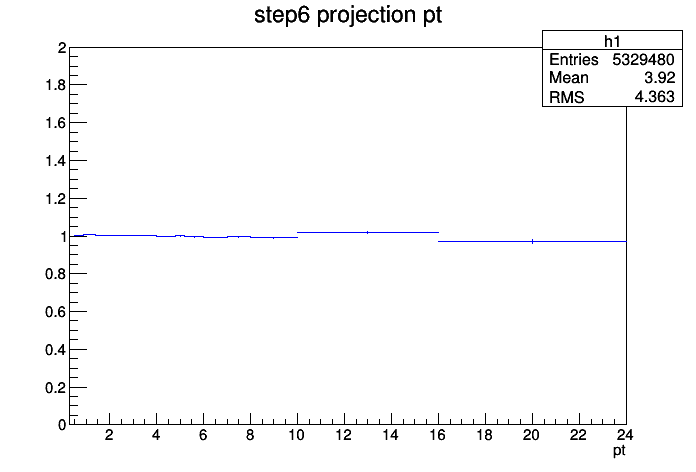
\includegraphics[width=0.8\linewidth]{figures/Effs/RatioEff_FiveSpecies.png}
	\caption{1D (vs $\pt$) tracking efficiency map for standard track selection, evaluated on f2b samples (blue) and f2a samples (red) on top panel, and their ratios on bottom panel.}
	\label{fig:trackeff}	
\end{figure}

\newpage
Details of cuts at event level and particle/track selection at different steps are listed in Table ~\ref{table:effCuts} . \\
\begin{table}[h]
\small
\centering % used for centering table

\begin{tabular}{  p{5cm} |  p{8.5cm} }
 \\
  \multirow{1}{*}{\large \textbf {MC Generated }} \\
\hline
\\
     Stages         &              Cuts \\
\hline\hline & \\		            	
  1.MC Part with Generated Cuts         &    {\textbf {After Event Selection}}\\
																		   & Charge\\
																		    & PDG Code\\
														  				  & Physical Primary \\

   2. MC Part with Kine Cuts         &              {\textbf {Kinematics Cuts }}\\
															    & -0.8$\textless \eta \textless  0.8$\\
															    & $\pt$ $\textgreater$ 0.3 (GeV/$c$)\\

&		\\            	


\multirow{1}{*}{\large \textbf {MC Reconstructed }} & \\
\hline


\hline & \\		            	                        	
4. Reco tracks        &                             {\textbf {After Event Selection}}\\
															   & Physical Primary \\
															
															
5. Reco tracks with Kine Cuts         &               {\textbf  {Kinematics Cuts }}\\
															    & -0.8$\textless \eta \textless  0.8$\\
															    & $\pt$ $\textgreater$ 0.3 (GeV/$c$)\\



6. MC true with Quality Cuts         &      			      {\textbf  {Quality Cuts }} \\
																	&SetRequireSigmaToVertex(kFALSE) \\
																	&SetDCAToVertex2D(kFALSE) \\
																	&SetMinNCrossedRowsTPC(70)\\
																	&SetMinRatioCrossedRowsOverFindableClustersTPC(0.8)\\
																	&SetMinNClustersITS(2)\\
																	&SetMaxChi2PerClusterTPC(4)\\
																	&SetMaxDCAToVertexZ(1) \\
																	&SetMaxDCAToVertexXY(1) \\
																	&SetRequireTPCRefit(TRUE) \\
																	&SetRequireITSRefit(FALSE) \\

7. Reco tracks with Quality Cuts         &             {\textbf  {Same as step 6}} \\

 &\\		            	            		

 \hline \hline
 \\
\end{tabular}
\caption{\large {The list of event and particle/track selection cuts used in the estimation of single track efficiency}} % title of Table
\label{table:effCuts}	
\end{table}

{\bf \large (ii) D meson efficiency} - Due to limited statistics, the correlation analysis is performed in quite wide $\pt$ bins and in each of them the reconstruction and selection efficiency of D mesons is not flat, in particular in the lower $\pt$ region. We correct for the $\pt$ dependence of the trigger efficiency within each p$_\mathrm{T}$-bin.

This correction is applied online, by using a map of D meson efficiency as a function of $\pt$ and event multiplicity (in terms of SPD tracklets in $|\eta|<1$) extracted from the enriched Monte Carlo sample LHC17d2a$\_$fast$\_$new. The $\eta$ dependence was neglected due to the statistics of the available Monte Carlo sample, which rule out the possibility of performing a 3D study.

To properly count the number of trigger particles used to normalize the correlation distributions, $N_\text{trig}$, each D meson is weighted with the inverse of its efficiency
in the invariant mass distribution. The main role of the correction for the D meson efficiency is to account for the $\pt$ dependence of the correlation distribution within a given D meson $\pt$ interval. Indeed, only the $\pt$ shape of the D meson efficiency within the correlation $\pt^{\rm trig}$ ranges is relevant while the average value
in the $\pt$ range is simplified due to the normalization of the correlation distribution to the number of trigger particles.

Efficiency plots for $\Dzero$, $\Dplus$ and $\Dstar$ mesons are shown in Figs.~\ref{fig:dEffPrompt} and ~\ref{fig:dEffFD}.

\begin{figure}[!htp]     %da c
	\centering
%Marianna
    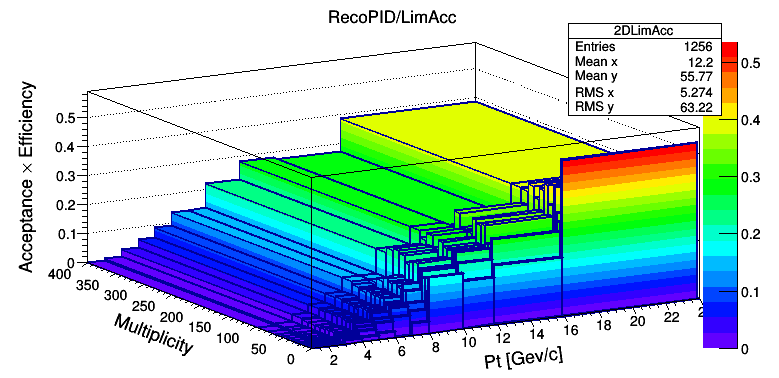
\includegraphics[width=.48\linewidth]{figures/Effs/EfficiencyMap_2D_DPlus_c_Ref_wLimAcc_Plot.png}
	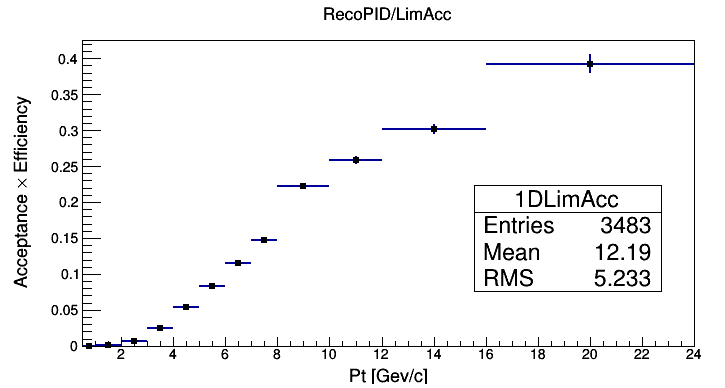
\includegraphics[width=.48\linewidth]{figures/Effs/EfficiencyMap_1D_DPlus_c_Ref_wLimAcc_Plot.png}  % by Fabio
	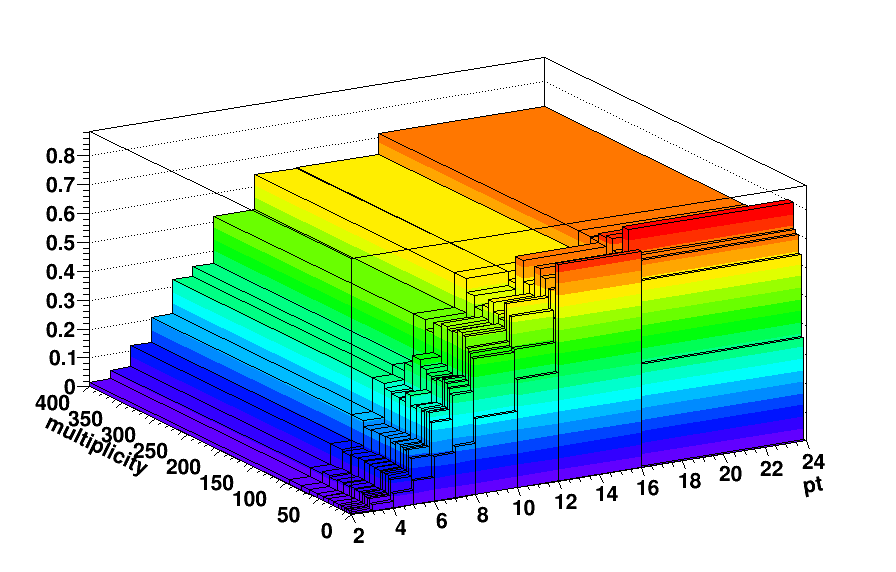
\includegraphics[width=.48\linewidth]{figures/Effs/EfficiencyMap_2D_DStar_c_Ref_wLimAcc_Plot.png}
	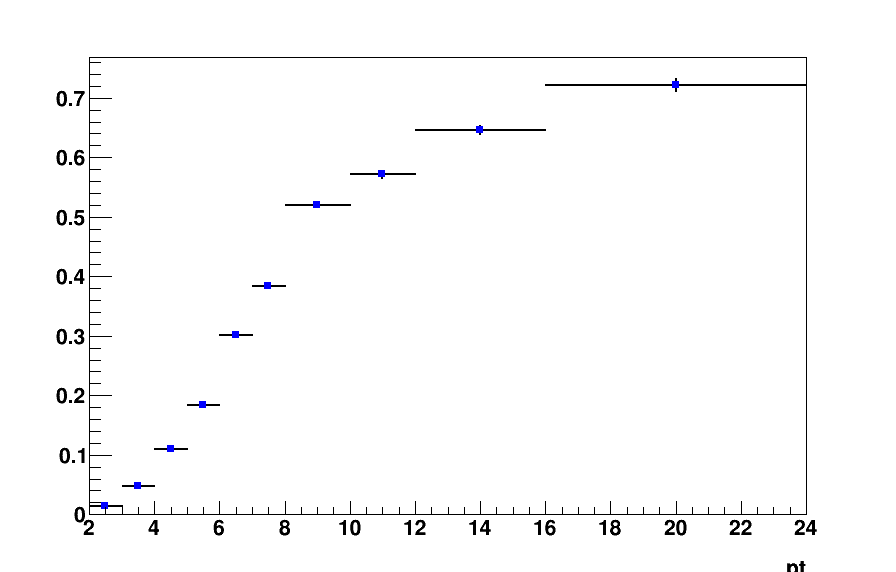
\includegraphics[width=.48\linewidth]{figures/Effs/EfficiencyMap_1D_DStar_c_Ref_wLimAcc_Plot.png}  % by Fabio
	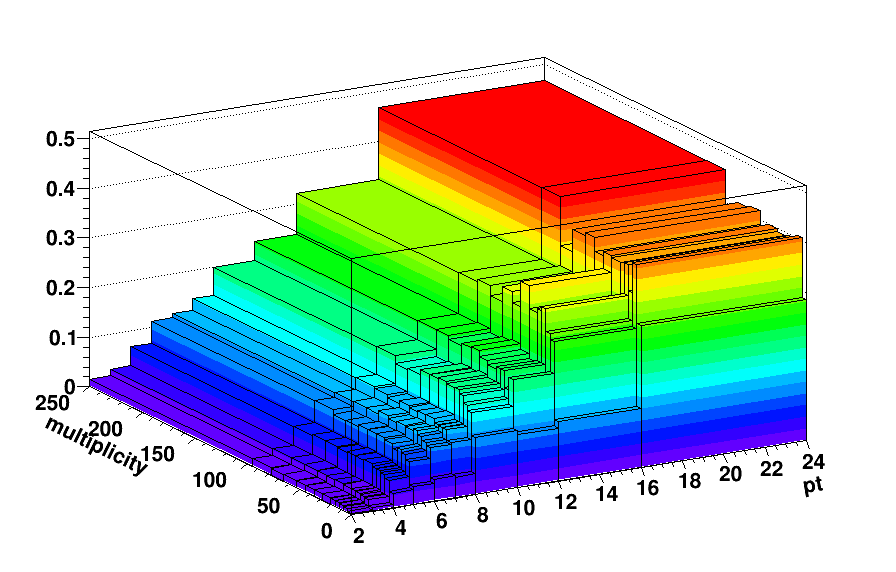
\includegraphics[width=.48\linewidth]{figures/Effs/EfficiencyMap_2D_Dzero_c_Ref_wLimAcc_Plot.png}
	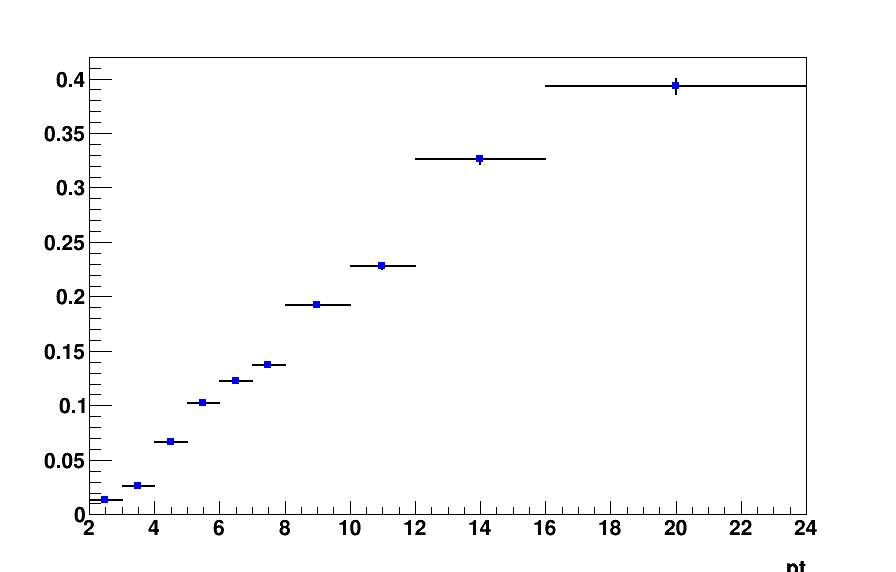
\includegraphics[width=.48\linewidth]{figures/Effs/EfficiencyMap_1D_Dzero_c_Ref_wLimAcc_Plot.png}  % by Fabio
	
	%\includegraphics[width=.30\linewidth]{figures/D0Eff_ProjMult_3to4GeV.png}
	%\includegraphics[width=.30\linewidth]{figures/D0Eff_ProjMult_5to6GeV.png}
	%\includegraphics[width=.30\linewidth]{figures/D0Eff_ProjMult_8to12GeV.png}
\caption{Top panel: ($\pt$, multiplicity) dependence (left) and $\pt$  dependence (right) of prompt $\Dplus$ meson efficiency.
Mid panel: ($\pt$, multiplicity) dependence (left) and $\pt$  dependence (right) of prompt $\Dstar$ meson efficiency.
Bottom panel: ($\pt$, multiplicity) dependence (left) and $\pt$  dependence (right) of prompt $\Dzero$ meson efficiency.
%s: multiplicity dependence of $D^0$ meson efficiency for three $D^0$ p$_\mathrm{T}$ ranges: 3-4 GeV/$c$ (left), 5-6 GeV/$c$ (center), 8-12 GeV/$c$ (right). For tracklet multiplicity$>$ 120, due to the limited statistics, the efficiency value is fixed to the one obtained for 90$<$tracklet multiplicity$<$120.
}
	\label{fig:dEffPrompt}	
\end{figure}

\begin{figure}[h]   %da B
	\centering
	%Marianna
		  % by Fabio
	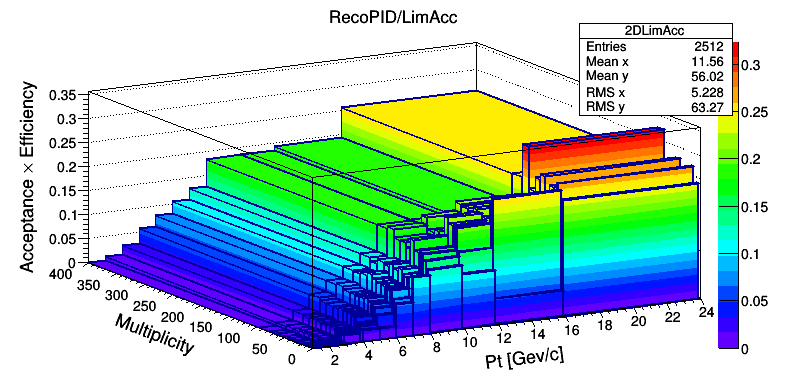
\includegraphics[width=.48\linewidth]{figures/Effs/EfficiencyMap_2D_DPlus_b_Ref_wLimAcc_Plot.png}
	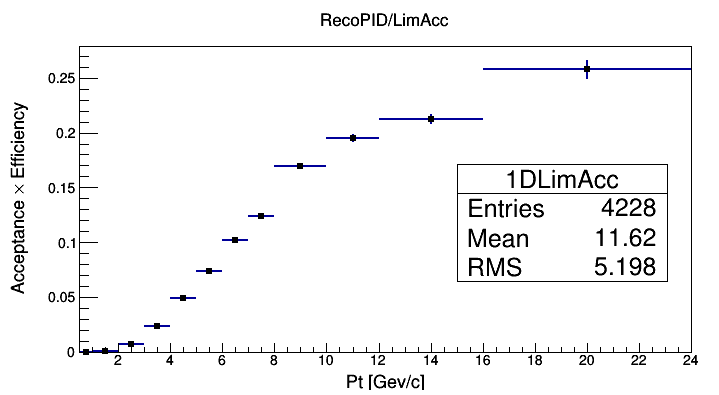
\includegraphics[width=.48\linewidth]{figures/Effs/EfficiencyMap_1D_DPlus_b_Ref_wLimAcc_Plot.png}
	  % by Fabio
	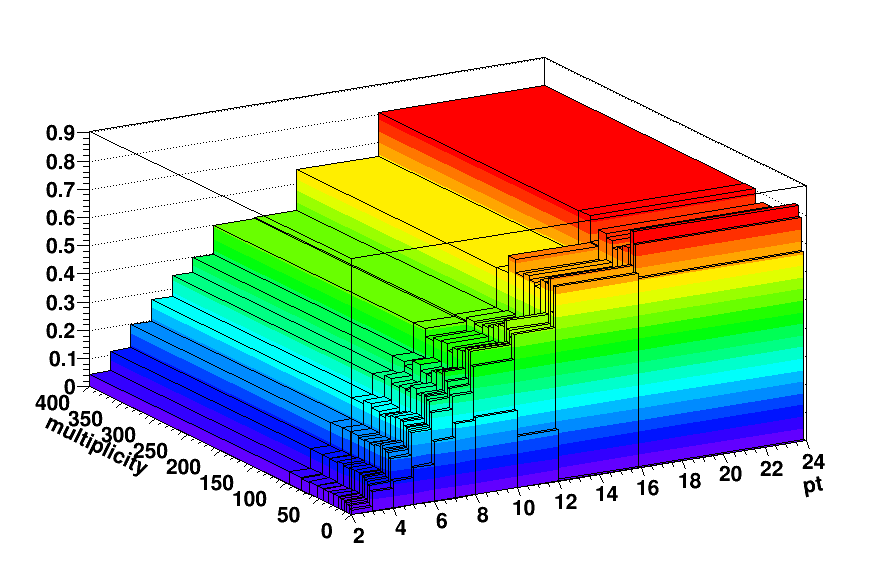
\includegraphics[width=.48\linewidth]{figures/Effs/EfficiencyMap_2D_DStar_b_Ref_wLimAcc_Plot.png}
	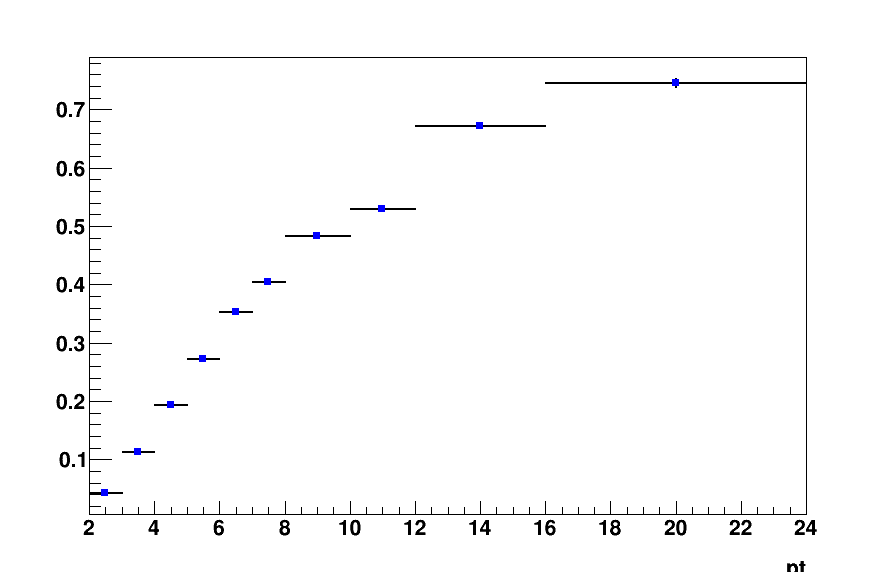
\includegraphics[width=.48\linewidth]{figures/Effs/EfficiencyMap_1D_DStar_b_Ref_wLimAcc_Plot.png}
	  % by Fabio
	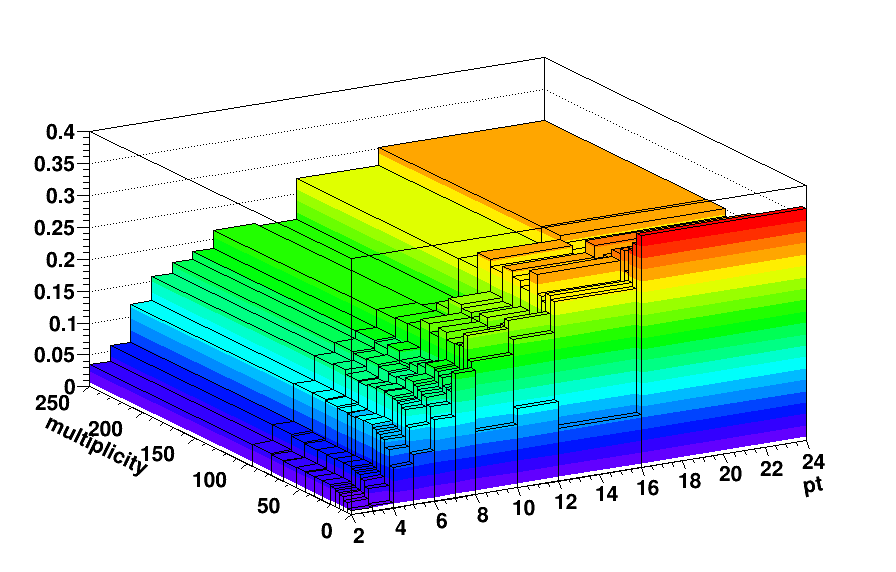
\includegraphics[width=.48\linewidth]{figures/Effs/EfficiencyMap_2D_Dzero_b_Ref_wLimAcc_Plot.png}
	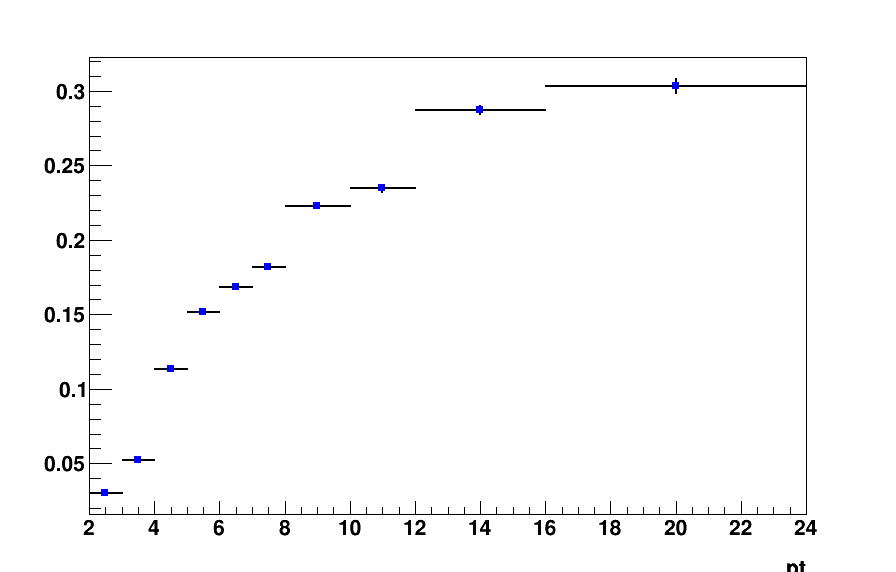
\includegraphics[width=.48\linewidth]{figures/Effs/EfficiencyMap_1D_Dzero_b_Ref_wLimAcc_Plot.png}
	\caption{Top panel: ($\pt$, multiplicity) dependence (left) and $\pt$ dependence (right) of feed-down $\Dplus$ meson efficiency.
Mid panel: ($\pt$, multiplicity) dependence (left) and $\pt$ dependence (right) of feed-down $\Dstar$ meson efficiency.
Bottom panel: ($\pt$, multiplicity) dependence (left) and $\pt$ dependence (right) of feed-down $\Dzero$ meson efficiency.}
	\label{fig:dEffFD}	
\end{figure}
\clearpage

It was observed that multiplicity dependence of the efficiency does not bias the extraction of the signal yield from the invariant mass distributions (which, as anticipated, are also weighted in the same manner). In addition, the multiplicity dependence of the efficiencies (shown for the $\Dzero$, in integrated $\pt$ range, in Fig. \ref{fig:DeffY}) is rather flat in the range 20-80 tracklets, where about 90\% of the reconstructed D-mesons are found, which explains why it has a negligible effect on the correlation distributions on this data sample.
\begin{figure}[h]   %da B
	\centering
	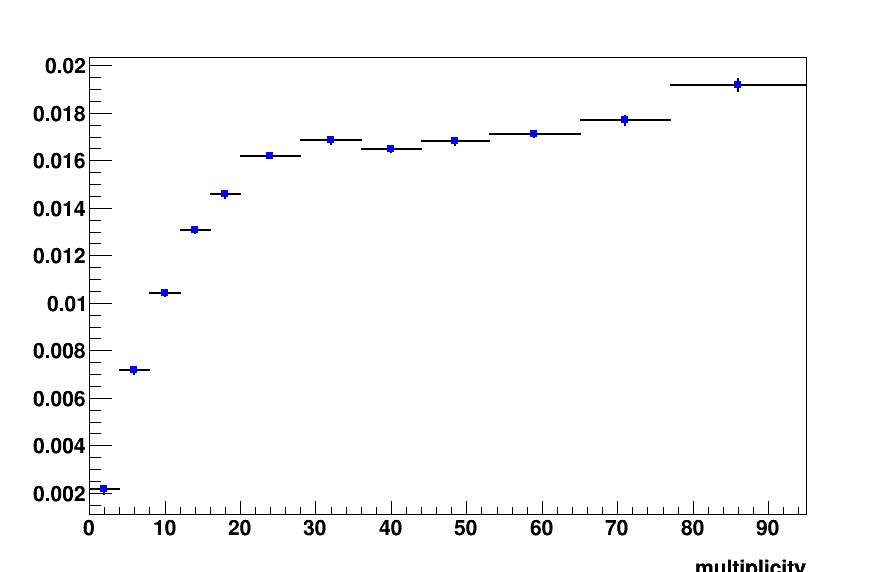
\includegraphics[width=.48\linewidth]{figures/Effs/EfficiencyMap_1D_Dzero_c_RefPtBins_Ydep_wLimAcc_Plot.png}
\caption{Prompt $\Dzero$ meson efficiency as a function of multiplicity (SPD tracklet in $|\eta|<1$).}
	\label{fig:DeffY}	
\end{figure}
\clearpage 


\subsubsection{Correction for bias on B to D decay topologies}
\input{./Sections/3Analysis_Strategy/MCclosureModulation.tex}

\subsubsection{Secondary track contamination}
\input{./Sections/3Analysis_Strategy/Secondaries.tex}

\subsubsection{Beauty feed-down}
\input{./Sections/3Analysis_Strategy/BeautyFeedDown.tex}


\newpage
\section{Systematic uncertainties on $\Delta\varphi$ correlation distributions}
\input{./Sections/4Systematic/SysUnc_AnalConst.tex}

\newpage
\section{Results}
The procedure for, after having evaluated all the needed correction, is totally equivalent to that described in Section 5.
As a quick reminder, the weighted average of the azimuthal correlation distributions for the three D-meson species are evaluated for each kinematic range under study, and a fit function (composed of a double Gaussian for the near- and away-side peak and a constant baseline) is applied to the average distribution, in order to extract quantitative observables as the NS and AS associated yield and widths.
Of course, the procedure is performed independently on each of the three centrality classes, and a comparison of the correlation distributions (after the baseline subtraction) and of the NS and AS peak observables is done.
The results of the analysis for each centrality class, and of the comparison, are shown in the following.

\subsubsection{Single-meson azimuthal correlation distributions}
- mostrare mesoni singoli da script pre-average

\subsubsection{Average-D correlation distributions}
- come da titolo

\subsubsection{Observables from fit to correlation distributions}


In the following:
\textit{\textbf{SHOW FIT OBSERVABLES AND THE PLOTS OF THEIR SYST UNCERTAINTIES!}}

\subsubsection{Plots proposed for preliminaries}
- mostra quelli da approvare 

%\newpage
%\section{Conclusions}
%\input{./Sections/6Conclusions/Conclusions.tex}

%\newpage
%\section{List of possible plots for preliminary}
%\input{./Sections/7Preliminary_Plots/Preliminary_plots_req.tex}

\newpage
\section{Bibliography}
\begin{thebibliography}{99}
\bibitem{ALICEDmespp7Tev} B. Abelev et al. [ALICE Collaboration], JHEP {\bf 01} (2012) 128
\bibitem{ALICEDhcorr} B. Abelev et al. [ALICE Collaboration], Eur. Phys. J. C (2017) 77:245
\bibitem{ALICEv2ppb} B. Abelev et al. [ALICE Collaboration], Phys.Lett. B719 (2013) 29-41
\bibitem{ALICEv2ppb2} B. Abelev et al. [ALICE Collaboration], Phys.Lett. B726 (2013) 164-177
\bibitem{ALICEv2HFe} https://aliceinfo.cern.ch/Figure/node/12130 (ALI-PREL-138003)
\bibitem{ALICEPbPbdih} ALICE Collaboration, arXiv:1609.06643 [nucl-ex]
\bibitem{NotepPb} https://aliceinfo.cern.ch/Notes/node/300
\bibitem{Notepp} https://aliceinfo.cern.ch/Notes/node/238
\bibitem{NoteD2HpPb} https://aliceinfo.cern.ch/Notes/node/201
\end{thebibliography} 



\end{document}
